\documentclass[10pt,a4paper]{article}

\usepackage[margin=0.82in]{geometry}
\usepackage[T1]{fontenc}
\usepackage{microtype}
\microtypesetup{expansion=false}
\usepackage{amsmath,amssymb}
\usepackage{booktabs,tabularx,array}
\usepackage{graphicx}
\usepackage{xcolor}
\usepackage{hyperref}
\usepackage{url}
\usepackage{titlesec}
\usepackage{tikz}
\usetikzlibrary{arrows.meta,positioning,fit,calc}
\usepackage{pgfplots}
\pgfplotsset{compat=1.18}
\usepackage{enumitem}
\graphicspath{{figures/}}

\hypersetup{colorlinks=true, linkcolor=black, urlcolor=blue, citecolor=black,
  pdftitle={Ariadne: Mapping the Way Back},
  pdfauthor={Ariadne project}}
\setlength{\parindent}{0pt}
\setlength{\parskip}{0.55em}
\setlist{nosep,leftmargin=1.4em}
\titleformat{\section}{\large\bfseries}{\thesection}{0.55em}{}
\titleformat{\subsection}{\normalsize\bfseries}{\thesubsection}{0.5em}{}
\renewcommand{\arraystretch}{1.12}
\newcolumntype{P}[1]{>{\raggedright\arraybackslash}p{#1}}
\newcommand{\code}[1]{\texttt{\small\detokenize{#1}}}
\newcommand{\ev}[1]{\url{#1}}
\newcommand{\indentedheading}[1]{\par\addvspace{0.65em}\noindent\hspace*{1em}\textbf{#1}\par\smallskip}

\title{\textbf{Ariadne: Mapping the Way Back}\\[0.3em]
\large A systems account of autonomous multi-agent collaborative visual mapping \\ and 3D construction under unreliable communication links}
\author{OpenCV AI Competition 2026 submission}
\date{Implementation and evidence snapshot: 26 October 2026}

\begin{document}
\maketitle

\begin{abstract}
A major structural collapse can leave people trapped in spaces responders cannot safely enter. The “golden 72 hours” is an imperfect but familiar reminder that useful information has to arrive while it can still shape the search. In these spaces, a camera feed leaves important questions hanging: where is the map backed by observations, can a person fit through an opening, and will the apparent shortest way back stay clear?

Ariadne studies how a team of autonomous visual agents can decide what to observe, what to share, and which measurements to trust as they build a common 3D model of the space under a shared mission budget. The pipeline starts with image registration, feature tracking, and stereo-inertial pose estimation. Each agent builds a local map and pose graph; over constrained links, agents exchange compact place-recognition cues, then check candidate connections with plausible geometry and robust consensus before they can reshape the shared map. The team uses that map to pick informative views, allocate exploration tasks, and plan a responder-sized route based on estimated clearance and risk. An LLM orchestration harness helps manage task-level decisions, with human review available when an action crosses the approved risk envelope. Gaussian splat reconstruction lets incident command inspect the space from viewpoints the agents never visited.

Experiments show clear gains across key parts of this chain: learned matching improves pose estimation over an ORB baseline across the tested EuRoC flights; stereo-inertial mapping reaches the comparison class of established systems; robust collaboration resolves severe perceptual aliasing while preserving tested true map connections; and evaluated egress routes agree with ground-truth passability. Ariadne takes its name from the princess who gave Theseus the thread to trace his way through the Labyrinth. Its thread is made of observations, verified geometry, and a route that can lead responders in, and guide them home.
\end{abstract}

\section{The Problem: Finding a Way Through the Labyrinth}

After a collapse, the spaces that matter most may be the ones a human cannot safely enter: narrow voids, unstable floors, dark corridors, rooms cut off by rubble, and routes whose open-looking entrances hide an impassable pinch point. Responders need more than a camera feed. They need to know where the map is backed by observations, whether two agents are describing the same corridor, whether a person can fit through it, and whether the route back out is still viable.

Ariadne is for incident-command teams and search-and-rescue responders who need spatial decision support from small visual agents. The agents use stereo RGB, inertial measurements in the SLAM pipeline, and camera-mounted lighting. They build geometry and routes; identifying people and tracking their identities over time are outside the system’s purpose.

The “golden 72 hours” gives the problem a familiar frame. It is a rule of thumb, not a promise or a stopwatch for every incident, but it captures the practical pressure: information has to arrive in time to affect a decision. A detailed map that turns up after the search has moved on is mostly an archival achievement.

The name Ariadne comes from the Greek myth. Princess Ariadne gives Theseus a thread to find his way through the Labyrinth and back out after facing the Minotaur. Ariadne aims to give responders a thread of its own: a route grounded in what the agents have observed, updated as the picture changes, and clear about where the evidence runs thin.

The research question is practical: when sensing, movement, communication, energy, and mission time are all limited, which observation should the team acquire next, which relationship should it transmit, and which geometric evidence should be allowed to move the shared map? Our hypothesis was that uncertainty- and connectivity-aware coordination would outperform local coverage maximization under the same mission costs.

Ariadne follows that question from the camera to the route home. Image restoration and feature tracking feed stereo-inertial pose estimation; keyframes and landmarks form local maps, refined by bundle adjustment and pose-graph optimization. Agents exchange compact retrieval cues over limited links, prioritize candidate connections under a communication budget, and use geometric consensus to stop false matches from bending the shared map. That joint model helps the team choose informative views and allocate tasks. A volumetric map estimates clearance and risk, and a responder-scale planner searches for a viable way out. An orchestration harness helps choose among proposed tasks, with human review available when an action crosses the risk gate. Gaussian splats make the explored space easier to inspect.

The thread starts with perception and ends with a route. For a responder to follow it, the connections along the way have to hold.

\section{What was built}

The work began with a thin end-to-end build: a repeatable simulated mission that could produce camera and IMU data, estimate motion, record the run, and replay the same evidence. ROS~2 Jazzy and Gazebo Harmonic provide the mission environment; MCAP carries recorded sensor streams, trajectories, and scene ground truth into repeatable evaluation. This first thread made interfaces concrete early. Images, poses, maps, collaboration messages, planning outputs, and reconstruction chunks cross explicit data boundaries, so each layer can be exercised from a recorded run before it is joined to the next.

From that base, the visual path grew into a keyframe-based stereo-inertial estimator. It tracks features between frames, triangulates local landmarks, refines recent poses and points with windowed bundle adjustment, and connects keyframes in a pose graph. The estimator and graph optimizer are Ariadne implementations built from OpenCV~5 and Eigen primitives. EuRoC~\cite{euroc} and TUM sequences supply public-data checks; GTSAM serves as an independent test oracle for selected graph problems, not as a runtime dependency. The next section follows the front end from the initial ORB/LK build to the adopted tracking and place-recognition components, and the section after it details local stereo-inertial estimation.

The next layer let agents build partial maps separately, then decide which cross-agent evidence was worth communicating and which candidate joins could safely influence the shared graph. Experiments shaped the final choices: retrieval and matching are selective, messages are budgeted, and geometric checks reject inconsistent joins before global optimization. On the resulting map, a volumetric layer estimates observed support, clearance, and a structural-risk proxy. Candidate views are scored for exploration and assigned to agents; a separate responder-scale search finds a route to an exit through known traversable space. The communication, planning, and egress sections describe those layers and their measured limits in turn.

Two services sit above this deterministic core. An LLM harness can choose among planner proposals and issue constrained directives through an MCP-facing service; it does not estimate geometry or execute unchecked commands. A risk gate is designed to route qualifying actions to human review, while validation and fallback checks remain in ordinary code. Gaussian submaps provide an inspectable visual representation alongside the geometric map. Their live transport and browser display are demonstrated separately from GPU training, which was evaluated on a synthetic corridor. The later sections keep those evidence boundaries visible: the diagram summarizes the system’s connections, while each subsystem section states what its own experiments establish and what has not yet been demonstrated in one integrated mission.

\clearpage
\begin{figure}[p]
  \centering
  \vspace*{\fill}
  \makebox[\textwidth][c]{%
    \rotatebox[origin=c]{+90}{%
            \IfFileExists{ariadne_system_diagram.pdf}{%
                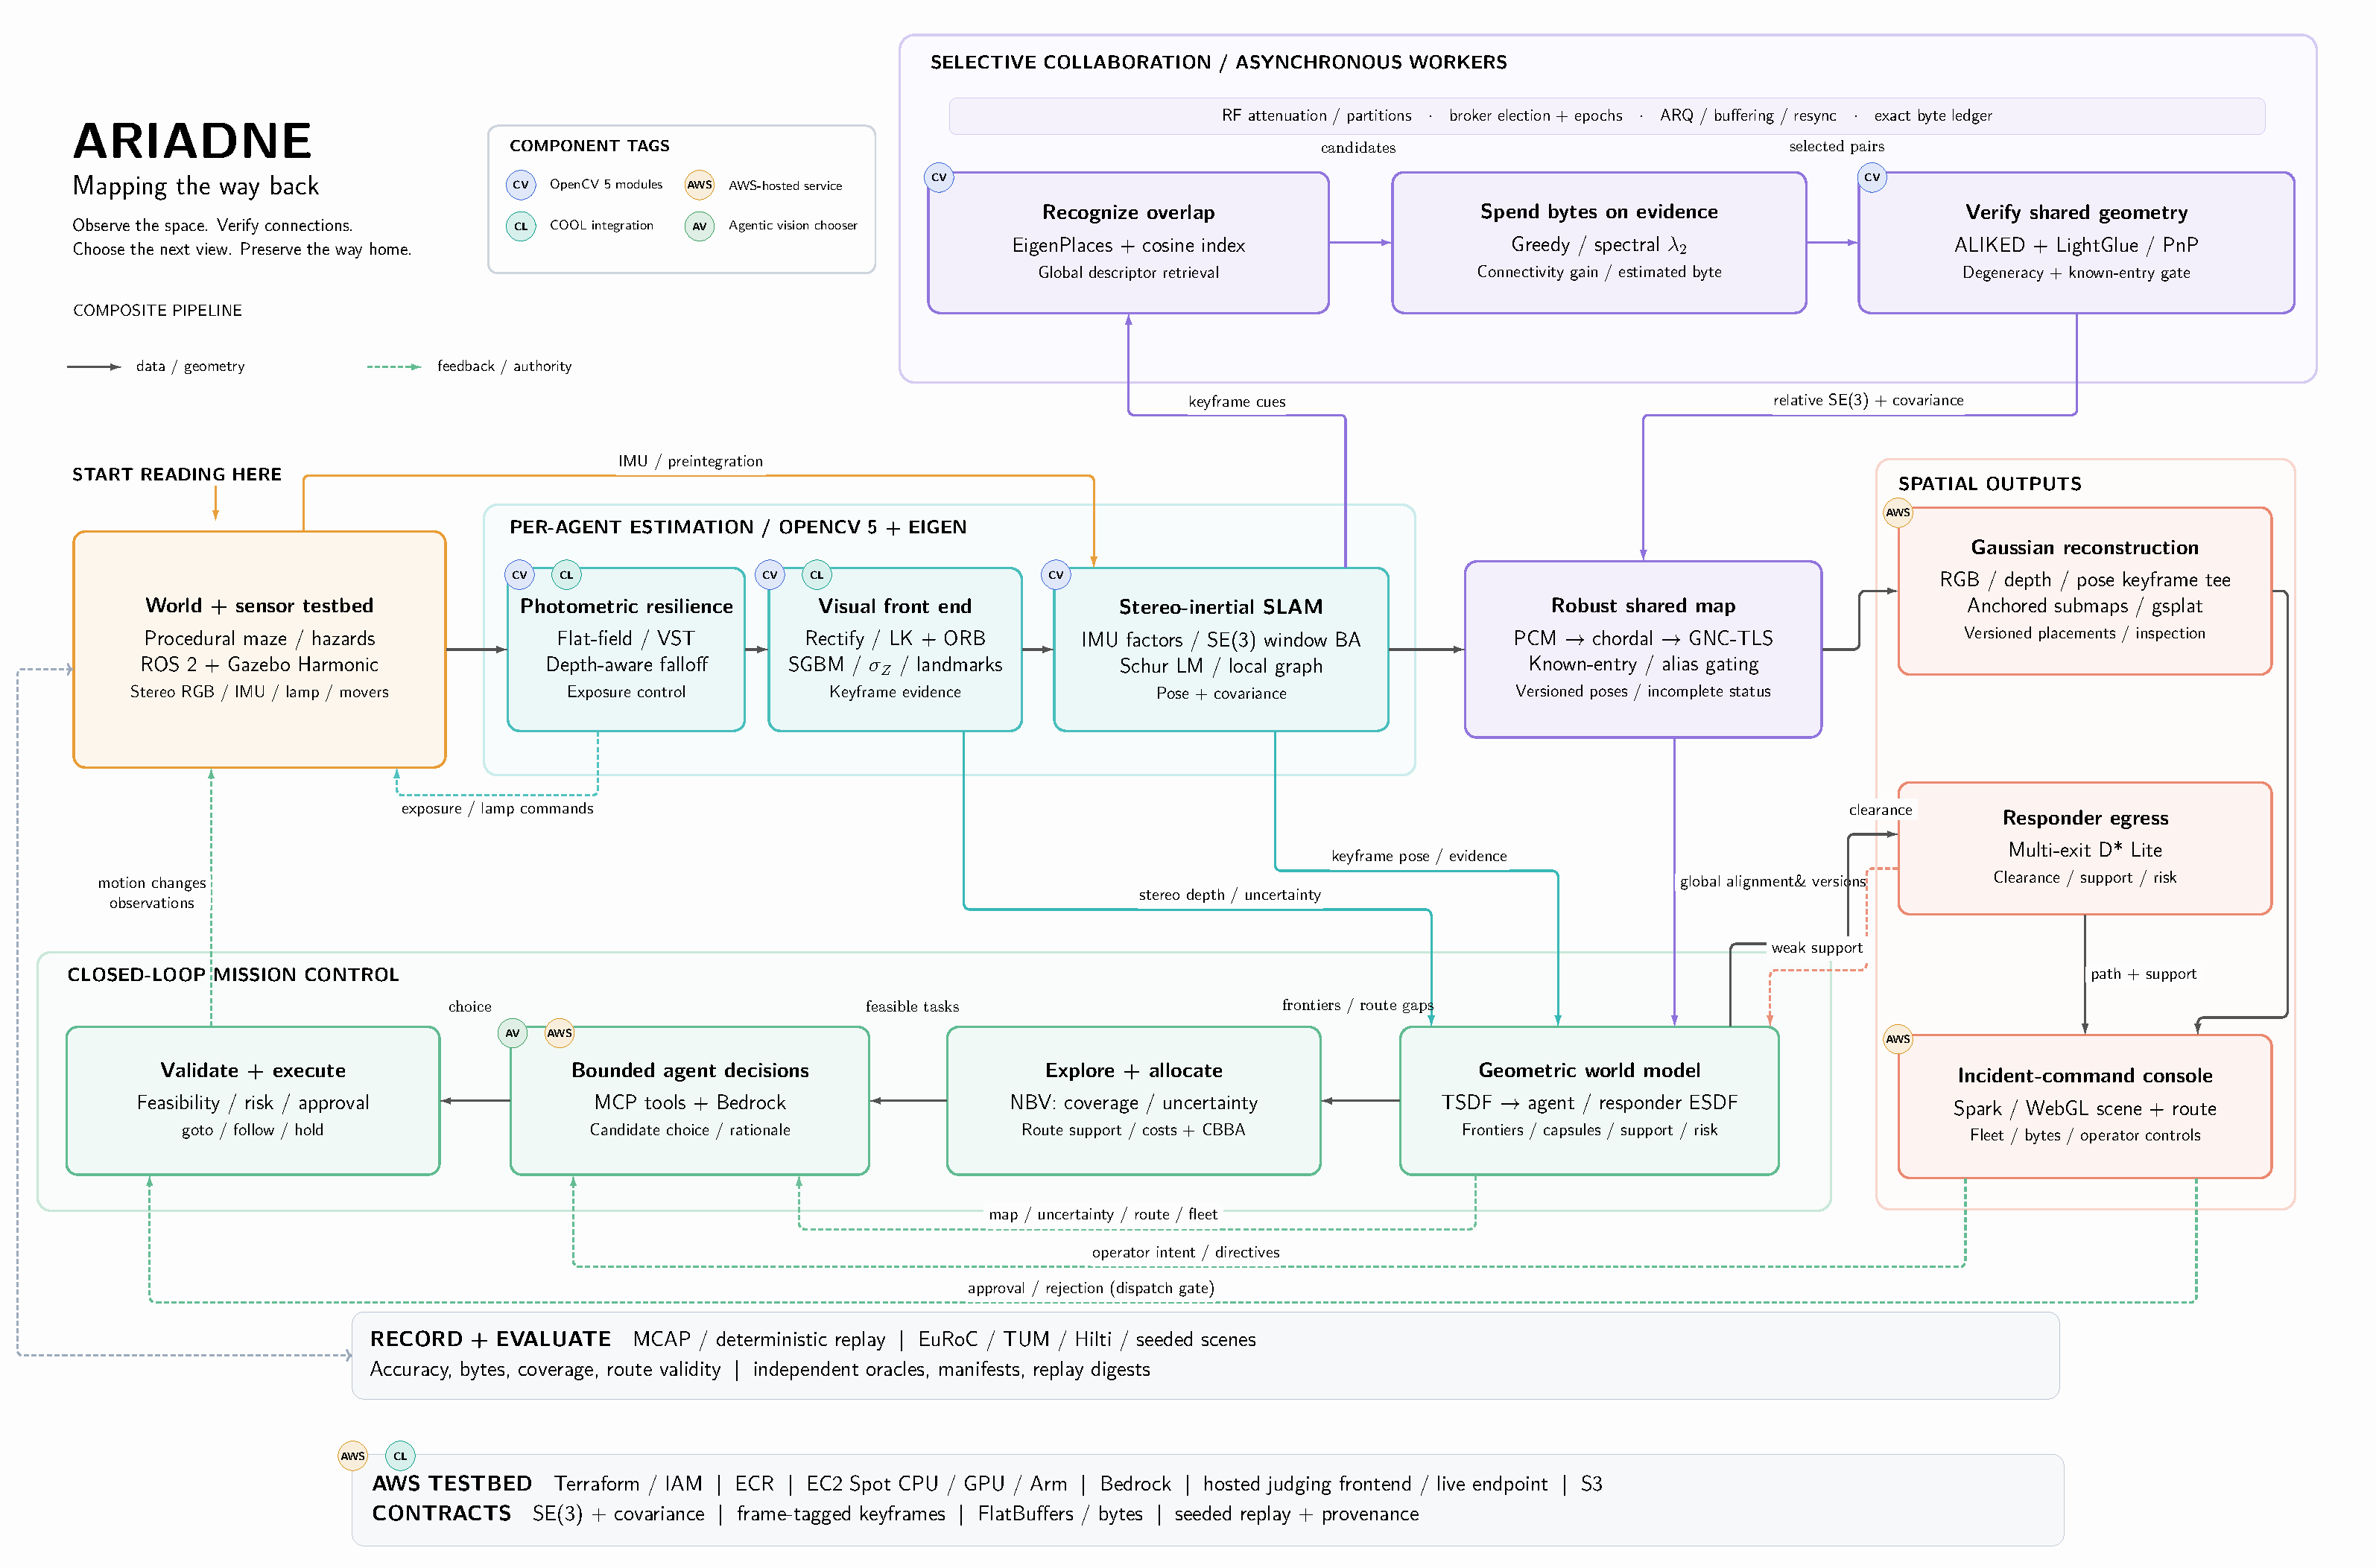
\includegraphics[width=0.90\textheight]{ariadne_system_diagram.pdf}%
            }{% 
                \fbox{\parbox[c][0.78\textheight][c]{0.86\textheight}{%
                    \centering\textit{System architecture diagram unavailable}%
                }}%
            }%
    }%
  }
  \par\vspace{0.6em}
  \caption{Ariadne's system architecture, from stereo-inertial sensing and
  OpenCV~5 estimation through selective collaboration, volumetric mapping,
  mission orchestration, responder egress, and Gaussian reconstruction.
  Solid arrows carry data and geometry; dashed arrows denote feedback,
  control, or replay. The lower rails identify evaluation and AWS services.}
  \label{fig:system}
  \vspace*{\fill}
\end{figure}
\clearpage

\section{Visual front end and place recognition}

Ariadne separates continuous visual tracking from the more expensive task of
recognizing a previously visited place. Pyramidal Lucas--Kanade (LK) carries
features between frames, while ORB replenishes tracks and supports landmark
recovery. At keyframes, EigenPlaces retrieves candidate overlaps; ALIKED and
LightGlue establish correspondences for selected pairs, which undergo geometric
verification before contributing constraints to the shared map. This division
concentrates learned inference where a successful recognition can correct
accumulated drift or connect two agents' maps.

\begin{figure}[ht]
\centering
\resizebox{0.94\linewidth}{!}{%
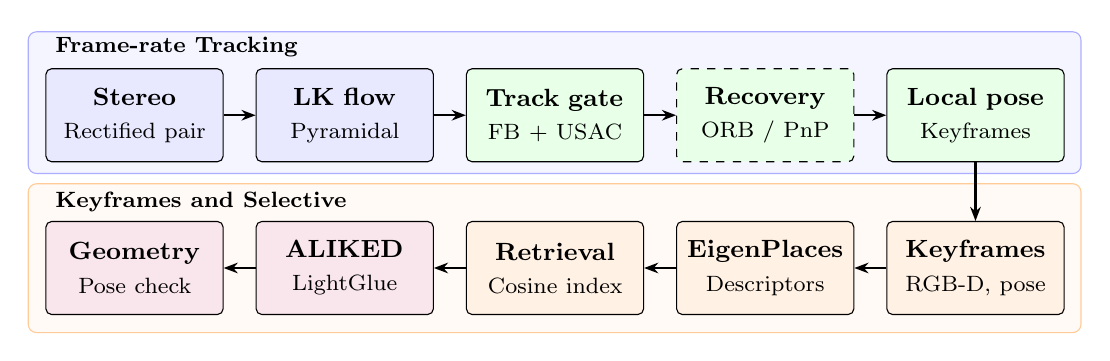
\begin{tikzpicture}[
  box/.style={
    draw,rounded corners=2pt,align=center,
    text width=2.00cm,minimum width=2.25cm,
    minimum height=1.18cm,
    inner xsep=2.4pt,inner ysep=3pt,font=\small
  },
  arr/.style={
    -{Stealth[length=1.8mm]},line width=.75pt
  },
  head/.style={
    font=\footnotesize\bfseries,anchor=west
  }
]

% Compact row backgrounds
\draw[draw=blue!32,fill=blue!4,rounded corners=3pt]
  (-.18,-.74) rectangle (13.19,1.06);
\draw[draw=orange!40,fill=orange!4,rounded corners=3pt]
  (-.18,-2.76) rectangle (13.19,-.87);

\node[head] at (.04,.87) {Frame-rate Tracking};
\node[head] at (.04,-1.10)
  {Keyframes and Selective};

% Frame-rate tracking
\node[box,fill=blue!9] (frames) at (1.17,0)
  {\textbf{Stereo}\\[1pt]
   {\footnotesize Rectified pair}};

\node[box,fill=blue!9] (lk) at (3.84,0)
  {\textbf{LK flow}\\[1pt]
   {\footnotesize Pyramidal}};

\node[box,fill=green!9] (gate) at (6.51,0)
  {\textbf{Track gate}\\[1pt]
   {\footnotesize FB + USAC}};

\node[box,fill=green!9,dashed] (upkeep) at (9.18,0)
  {\textbf{Recovery}\\[1pt]
   {\footnotesize ORB / PnP}};

\node[box,fill=green!9] (pose) at (11.85,0)
  {\textbf{Local pose}\\[1pt]
   {\footnotesize Keyframes}};

\draw[arr] (frames.east)--(lk.west);
\draw[arr] (lk.east)--(gate.west);
\draw[arr] (gate.east)--(upkeep.west);
\draw[arr] (upkeep.east)--(pose.west);

% Keyframe-only matching
\node[box,fill=orange!11] (kf) at (11.85,-1.94)
  {\textbf{Keyframes}\\[1pt]
   {\footnotesize RGB-D, pose}};

\node[box,fill=orange!11] (ep) at (9.18,-1.94)
  {\textbf{EigenPlaces}\\[1pt]
   {\footnotesize Descriptors}};

\node[box,fill=orange!11] (retrieve) at (6.51,-1.94)
  {\textbf{Retrieval}\\[1pt]
   {\footnotesize Cosine index}};

\node[box,fill=purple!10] (lg) at (3.84,-1.94)
  {\textbf{ALIKED}\\[1pt]
   {\footnotesize LightGlue}};

\node[box,fill=purple!10] (geom) at (1.17,-1.94)
  {\textbf{Geometry}\\[1pt]
   {\footnotesize Pose check}};

% Orthogonal connections
\draw[arr] (pose.south)--(kf.north);
\draw[arr] (kf.west)--(ep.east);
\draw[arr] (ep.west)--(retrieve.east);
\draw[arr] (retrieve.west)--(lg.east);
\draw[arr] (lg.west)--(geom.east);

\end{tikzpicture}%
}
\caption{Ariadne tracks and validates features on every
frame, replenishing ORB tracks and re-associating landmarks
with PnP when needed. At keyframes, EigenPlaces retrieves
candidate overlaps; ALIKED--LightGlue and geometric
verification run only on selected pairs.}
\label{fig:perception}
\end{figure}

The front end evolved through measurement. The initial ORB/LK pipeline was
followed by an OpenCV DNN implementation of XFeat, assembled from upstream
weights and checked against reference outputs. XFeat reduced tracking losses
but increased trajectory error on six of seven previously passing EuRoC
flights. Changes to keyframe cadence, descriptor matching, and landmark
re-association did not eliminate the regression. The adopted EuRoC
visual-odometry configuration therefore retains ORB, reserving learned
features for place recognition and selective pairwise matching
\cite{orb,xfeat,aliked,lightglue,eigenplaces}.

Each frame passes through three-level pyramidal LK with a $21$-pixel window,
forward/backward consistency checks, and seeded USAC fundamental-matrix
estimation to reject epipolar outliers. An $8\times6$ spatial grid distributes
up to $1{,}000$ ORB keypoints, with $400$ active tracks as the replenishment
target. When landmark-bearing tracks fall below $30$, recovery matches current
observations against healthy, untracked landmarks in the local window.
Mutual nearest-neighbour matching, a $0.75$ ratio test, and a Hamming-distance
cap of $50$ precede seeded PnP verification requiring at least $12$ inliers.
Recovered tracks consequently retain an established 3D observation history.

At each keyframe, EigenPlaces produces a unit-normalized, $256$-dimensional
descriptor. An exact cosine index retrieves candidate overlaps, which the
communication policy can prioritize by expected graph-connectivity gain and
transmission cost. Exact and approximate search returned identical top-ranked
places on all $297$ evaluated EuRoC queries; exact search required only
microseconds for thousands of descriptors. Selected pairs proceed to
ALIKED-n16, capped at $1{,}024$ keypoints at native image resolution, and
the nine-layer LightGlue matcher. The exported models reproduce upstream
keypoints within $10^{-4}$ pixels and yield identical LightGlue match sets.
Increasing the keypoint cap to $2{,}048$ brought no measured pose gain at
approximately $2.8\times$ the cost.

\begin{quote}\small
\textbf{Verification path.}
LK tracking and ORB recovery maintain local landmark continuity.
EigenPlaces proposes revisits; ALIKED--LightGlue supplies correspondences;
seeded geometric estimation, PnP, degeneracy checks, and robust graph
consistency determine which proposed connections can influence the map.
\end{quote}

OpenCV 5 supplies the computational primitives:
\code{cv::buildOpticalFlowPyramid} and \code{cv::calcOpticalFlowPyrLK}
for tracking; \code{cv::ORB}, \code{cv::ALIKED}, and
\code{cv::LightGlueMatcher} for features and matching;
\code{cv::dnn::Net} for EigenPlaces and the XFeat experiment;
and seeded USAC through \code{cv::findFundamentalMat} and PnP.
Ariadne implements track management, landmark re-association, descriptor
indexing, inference wrappers, and geometric acceptance policy.
The pinned OpenCV 5.0.0 build lacks a native \code{cv::XFeat} class;
its network was assembled over OpenCV DNN primitives \cite{opencv5}.

On $4{,}815$ EigenPlaces-retrieved EuRoC keyframe pairs across $11$
flights, including $676$ ground-truth-positive pairs, ALIKED--LightGlue
increased pose AUC at $10^\circ$ from \textbf{$0.284$} for ORB to
\textbf{$0.607$}, matching or exceeding ORB on every flight.
Geometric average precision, scored against the fixed set of positives,
rose from \textbf{$0.303$ to $0.807$}; LightGlue contributed another
$0.042$ AUC over ALIKED with mutual-nearest-neighbour matching.
Four confidently incorrect essential-matrix verifications nevertheless
survived with $210$--$264$ inliers and rotation errors of
$37^\circ$--$59^\circ$. Their failure establishes the importance of the
downstream PnP, degeneracy, and consistency gates, particularly in
visually repetitive interiors.

For place retrieval, EigenPlaces achieved \textbf{$0.626$ R@1} at
$376\times240$, against $0.444$ for mean-bit descriptors and $0.167$
for random retrieval. On $61$ revisit queries from one clean simulator
scene, its $640\times360$ export reached $0.705$ R@1, with no observed
top-1 benefit from full resolution. Four-thread CPU measurements gave
p50 inference times of $311.8$\,ms for EigenPlaces at $640\times360$,
$1{,}998.6$\,ms for ALIKED at $1280\times720$, and $921.0$\,ms for a
warm LightGlue pair. These costs justify the event-driven learned path:
LK sustains frame-to-frame estimation, while expensive recognition is
invoked when its evidence can materially change the map. ORB remains
the matched pairwise baseline here; the complete estimator is compared
with published stereo-inertial systems in the following section.


\begin{figure}[t]
  \centering
  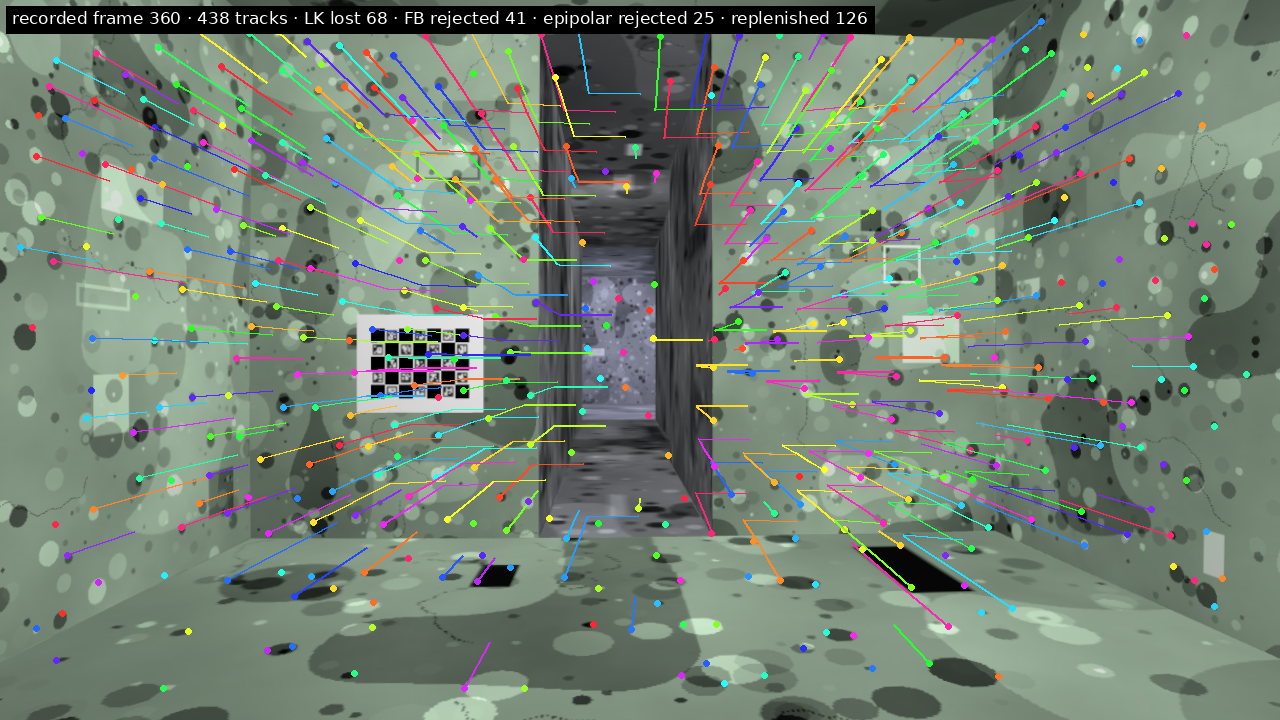
\includegraphics[width=\linewidth]{fig_tracking.png}
  \caption{The front end on a recorded agent-0 camera frame (lit maze, recorded run \code{c51ab2}). Each colour is
  one track; the trail joins its positions over the previous sampled frames. Tracks were replayed offline with
  OpenCV~5 \code{calcOpticalFlowPyrLK} on every 20th recorded frame (window 21, four pyramid levels, forward--backward
  threshold 0.5\,px, \code{findFundamentalMat} RANSAC at 1\,px), and the banner shows that frame's track
  statistics. Script: \code{figures/src/make\_stills.py}.}
  \label{fig:tracking}
\end{figure}

\section{Stereo-inertial estimation and local SLAM}

\indentedheading{Estimator architecture}

Ariadne combines stereo geometry with inertial motion estimates in a sliding-window visual-inertial estimator. Stereo supplies metric depth; IMU preintegration carries rotation, velocity, and position information between keyframes. The estimator maintains a local landmark map and emits pose and covariance estimates to a local SE(3) pose graph.

\begin{figure}[ht]
\centering
\resizebox{0.94\linewidth}{!}{%
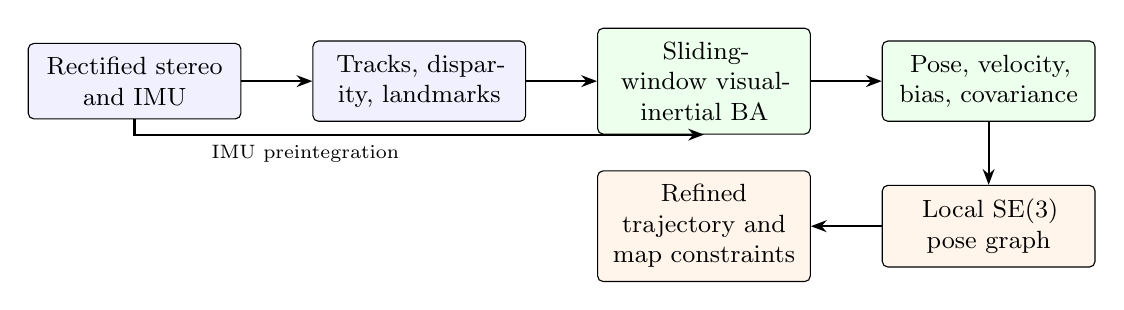
\begin{tikzpicture}[
  node distance=8mm and 9mm,
  box/.style={draw,rounded corners=2pt,align=center,inner sep=5pt,
    text width=2.35cm,minimum height=0.78cm,font=\small},
  arr/.style={-{Stealth[length=2mm]},thick}
]
\node[box,fill=blue!6] (sensor) {Rectified stereo and IMU};
\node[box,fill=blue!6,right=of sensor] (vision) {Tracks, disparity, landmarks};
\node[box,fill=green!7,right=of vision] (ba) {Sliding-window visual-inertial BA};
\node[box,fill=green!7,right=of ba] (state) {Pose, velocity, bias, covariance};
\node[box,fill=orange!8,below=of state] (graph) {Local SE(3) pose graph};
\node[box,fill=orange!8,left=of graph] (map) {Refined trajectory and map constraints};
\draw[arr] (sensor)--(vision); \draw[arr] (vision)--(ba);
\draw[arr] (sensor.south) |- node[pos=0.65,below,font=\scriptsize]{IMU preintegration} (ba.south);
\draw[arr] (ba)--(state); \draw[arr] (state)--(graph); \draw[arr] (graph)--(map);
\end{tikzpicture}%
}
\caption{Stereo and inertial measurements constrain a local sliding window; its pose and covariance outputs form odometry edges in the local pose graph.}
\label{fig:vio}
\end{figure}

\indentedheading{Stereo geometry and landmark management}

Ariadne matches rectified stereo images, estimates disparity with Semi-Global Block Matching, and triangulates landmarks in metric coordinates. Landmark admission checks parallax, depth, reprojection error, stereo uncertainty, and relative position uncertainty. Tracks that survive across keyframes add multi-view observations. After optimization, high-residual observations are removed; landmarks are culled according to whether they were observed when predicted visible.

Online row refinement compensates for residual vertical misalignment between cameras. On run V2\_01, we reduced the median stereo row residual from \textbf{1.46 px to 0.09 px}. Left-right exposure matching also helps preserve correspondences when the cameras' automatic exposure differs.

\indentedheading{Sliding-window visual-inertial optimization}

The adopted window contains ten keyframes. Each camera pose is represented on SE(3); full inertial mode adds world-frame velocity, gyro bias, and accelerometer bias. Visual residuals are reprojection errors in both rectified cameras. Consecutive keyframes receive preintegrated IMU factors and bias random-walk factors. Visual residuals use uncertainty weighting and a Huber loss.

A keyframe score combines translation, rotation, parallax, track loss, and pose uncertainty, with hard limits on track count and elapsed time. The oldest keyframe anchors the window gauge. Analytic Jacobians assemble the damped normal equations. Ariadne Schur-eliminates the independent 3D landmark blocks, solves the reduced pose system, and back-substitutes landmark updates. Selected covariance blocks are recovered through linear solves rather than an explicit inverse. When a keyframe leaves the window, its relative pose and transported covariance become an odometry edge for the local pose graph.

\indentedheading{Initialization and recovery}

IMU samples are preintegrated between keyframes using the on-manifold formulation of Forster et al.~\cite{forster}. Each inertial edge summarizes rotation, velocity, and position change, including propagated uncertainty and bias sensitivity. Initialization follows ten consecutive measured keyframes: Ariadne estimates gyro bias from visual and inertial rotations, solves for velocity, gravity, and accelerometer bias, then refines gravity magnitude.

Gravity is estimated at initialization and held fixed in the world frame while the window refines velocity and biases. We tested estimating gravity tilt independently in each window, but short-window tilt and accelerometer bias were weakly distinguishable; allowing both to drift made the trajectory less stable. The adopted solution keeps the initialized gravity direction fixed.

When tracking is lost, Ariadne records pose provenance and uses inertial and visual bridging to support recovery. Gyro-only rotation while lost was an earlier estimator mode; full preintegration in the window is the adopted EuRoC configuration.

\indentedheading{Implementation and validation}

OpenCV 5 supplies stereo disparity, triangulation, PnP, and the Levenberg--Marquardt driver. Ariadne implements the inertial model, residuals, analytic Jacobians, Schur backend, covariance handling, and local graph state. Eigen provides the reduced-system and graph factorizations.

\begin{table}[ht]
\centering
\small
\begin{tabular}{@{}P{2.8cm}P{4.3cm}P{8.7cm}@{}}
\toprule
\textbf{Operation} & \textbf{OpenCV 5 connection} & \textbf{Ariadne implementation} \\
\midrule
Stereo depth and geometry & \code{StereoSGBM}, \code{triangulatePoints}, \code{solvePnPRansac} & Landmark admission and uncertainty policy \\
Nonlinear optimization & \code{cv::detail::LevMarqBase} & Visual-inertial factors, analytic Jacobians, Schur elimination \\
Pose refinement checks & \code{solvePnPRefineLM}, \code{projectPoints} & Jacobian and solver cross-checks \\
IMU fusion & No OpenCV inertial primitive & Preintegration, initialization, bias and gravity estimation \\
\bottomrule
\end{tabular}
\caption{OpenCV provides geometry and the optimization driver; Ariadne supplies the visual-inertial estimation problem.}
\label{tab:vio-opencv}
\end{table}

Numerical checks agreed with independent references: the pose-graph solver matched GTSAM 4.3~\cite{gtsam} on \textbf{100/100} seeded synthetic graphs, with worst relative energy difference $1.5\times10^{-12}$. A one-free-pose bundle-adjustment case matched OpenCV's PnP refinement within \textbf{$1.3\times10^{-9}$ m} and \textbf{$2.8\times10^{-9}$ rad}. Estimator outputs were bit-identical across OpenCV thread-pool settings of 2, 5, and 16 threads for three trajectories of 4,001 poses each.

\begin{quote}\small
\textbf{Estimator loop.} Initialize velocity, gravity, and biases from ten measured keyframes. For each frame, track stereo features and validate landmarks. When the keyframe policy fires, add the pose, landmarks, and preintegrated IMU factor; run up to ten damped LM iterations with landmark Schur elimination; recover selected pose covariance; and emit a relative-pose odometry edge. During tracking loss, retain pose provenance and use the configured visual and gyro bridging.
\end{quote}

\indentedheading{EuRoC evaluation}

The loop-closed and VIO-only rows below come from the \textbf{same 11-flight run}, with the same seed, keyframe-refined ATE, and alignment procedure. Ariadne's VIO-only row reproduces the earlier run to four decimal places. ATE is computed over the refined trajectory after SE(3) alignment, without scale adjustment. The loop-closed system improves mean ATE from \textbf{0.120 m to 0.066 m}.

\begin{table}[ht]
\centering
\small
\begin{tabular}{@{}lrrrr@{}}
\toprule
\textbf{EuRoC flight} & \textbf{Ariadne VIO} & \textbf{Ariadne + loops} & \textbf{ORB-SLAM3} & \textbf{Class ceiling} \\
\midrule
MH\_01 & 0.068 & \textbf{0.021} & 0.036 & 0.166 \\
MH\_02 & 0.044 & \textbf{0.028} & 0.033 & 0.152 \\
MH\_03 & 0.099 & \textbf{0.033} & 0.035 & 0.125 \\
MH\_04 & 0.223 & \textbf{0.046} & 0.051 & 0.280 \\
MH\_05 & 0.140 & \textbf{0.044} & 0.082 & 0.284 \\
V1\_01 & 0.054 & 0.038 & 0.038 & 0.076 \\
V1\_02 & 0.047 & \textbf{0.027} & 0.014 & 0.110 \\
V1\_03 & 0.329 & 0.288 & 0.024 & 0.120 \\
V2\_01 & 0.039 & \textbf{0.030} & 0.032 & 0.070 \\
V2\_02 & 0.110 & 0.071 & 0.014 & 0.100 \\
V2\_03 & 0.169 & 0.097 & 0.024 & 0.190 \\
\midrule
\textbf{Mean} & \textbf{0.120} & \textbf{0.066} & \textbf{0.035} & \textbf{0.138} \\
\bottomrule
\end{tabular}
\caption{EuRoC RMS ATE in metres. The per-flight class ceiling is the worst published result among ORB-SLAM3, VINS-Fusion, Kimera, and BASALT; the aggregate ceiling is 0.138 m.}
\label{tab:vio-euroc}
\end{table}

By that explicit comparison rule, Ariadne VIO is within the published class on \textbf{9/11} flights, and the loop-closed system on \textbf{10/11}. The loop-closed system matches or improves on ORB-SLAM3's published per-flight result on \textbf{7/11} flights. Its mean remains above ORB-SLAM3's published 0.035 m mean due to the outlier run V1\_03 skewing the mean.

This is a published-baseline comparison, not a same-binary rerun: Ariadne's figures are a single seed-1 run, while reference numbers are taken from the systems' published results. ORB-SLAM3 is a full SLAM system, and BASALT's reported mean covers ten flights; these differences matter when interpreting the table. The visual-inertial formulation, comparison systems, and dataset are described in the original papers~\cite{euroc,orbslam3,forster,basalt,kimera}.
\begin{figure*}[t]
  \centering
  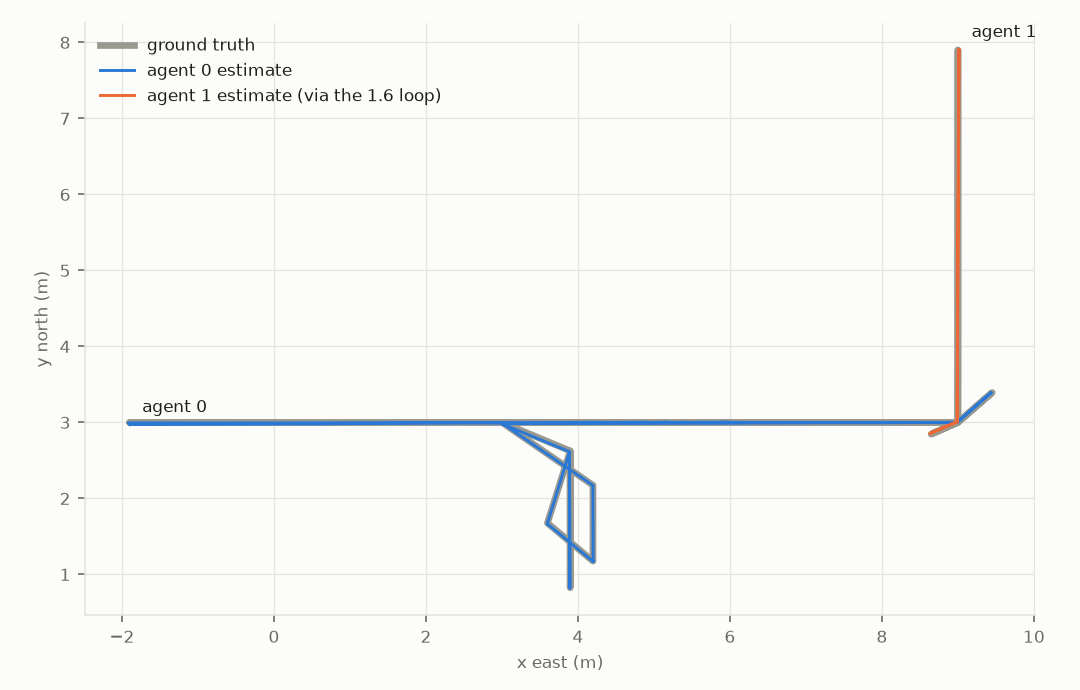
\includegraphics[width=0.49\textwidth]{fig_premerge_trajectories.png}\hfill
  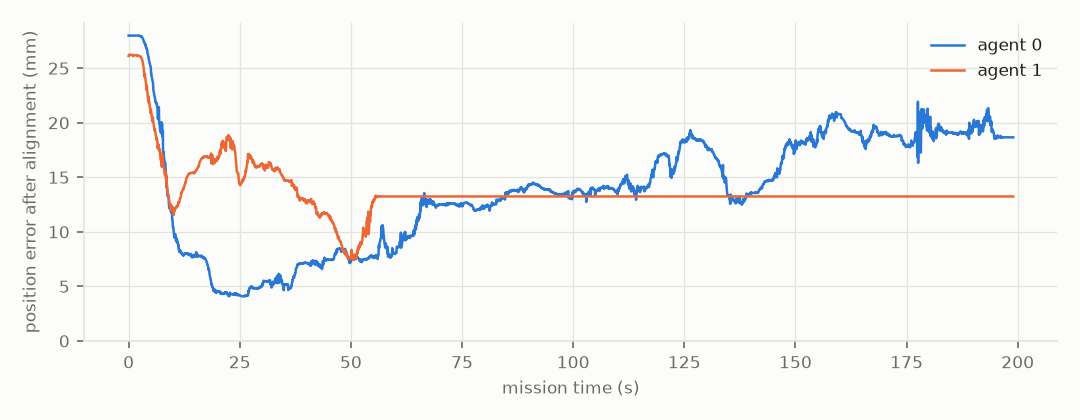
\includegraphics[width=0.49\textwidth]{fig_premerge_ate.png}
  \caption{Two-agent simulated mission from the AWS pre-merge gate (c7i spot, run \code{20261024T083919Z-cpux86-73e3fa},
  54/54 checks). Left: estimated trajectories over ground truth, with agent~1 placed through the inter-agent loop.
  Right: position error after alignment over the 200\,s mission, in millimetres.}
  \label{fig:premerge}
\end{figure*}

\section{Communication-aware collaborative mapping}

A shared map is only as reliable as the connections between its local maps.
Finding those connections begins with recognizing overlapping places, continues
with deciding which evidence is worth transmitting, and ends with determining
which geometric constraints can safely reshape the shared graph. In collapsed
interiors, repeated corridors and similar openings make false connections
especially costly: one plausible but incorrect loop closure can displace an
entire agent trajectory. Ariadne couples communication selection with robust
estimation, accounting for serialized bytes, rejecting inconsistent geometry,
and preserving an explicitly incomplete map when connectivity is lost.

\indentedheading{Architecture and communication-aware selection}

Each agent maintains an independent stereo-inertial map and publishes compact
EigenPlaces descriptors when links permit. Candidate overlaps are ranked before
the broker requests ALIKED--LightGlue feature evidence. Feature payloads are
cached by keyframe, allowing several candidate edges to reuse one transmission.
This two-stage exchange reserves expensive correspondence data for potentially
useful connections and makes communication cost part of the mapping decision.

Ariadne evaluates candidate edges through their expected improvement to
pose-graph algebraic connectivity, $\lambda_2(L)$, the second-smallest
eigenvalue of the graph Laplacian. For an edge $e=(i,j)$ with expected weight
$w_e$, its first-order spectral gain is

\begin{equation}
    \Delta\lambda_2(e)
    \approx w_e(v_i-v_j)^2,
    \qquad
    s(e\mid S)=
    \frac{\Delta\lambda_2(e)}{c(e\mid S)},
    \label{eq:collab-spectral}
\end{equation}

where $v$ is the Fiedler vector and $c(e\mid S)$ is the marginal wire cost
given already selected exchanges $S$. The broker greedily selects high-scoring
candidates subject to the byte budget, with local one-swap refinement. A simpler
greedy policy and exact enumeration on small instances provide comparison
points. This follows the task-oriented exchange principle of Tian et
al.~\cite{tian2018near}, applied here to graph connectivity and measured
serialized traffic.

\begin{figure*}[t]
\centering
\resizebox{\linewidth}{!}{%
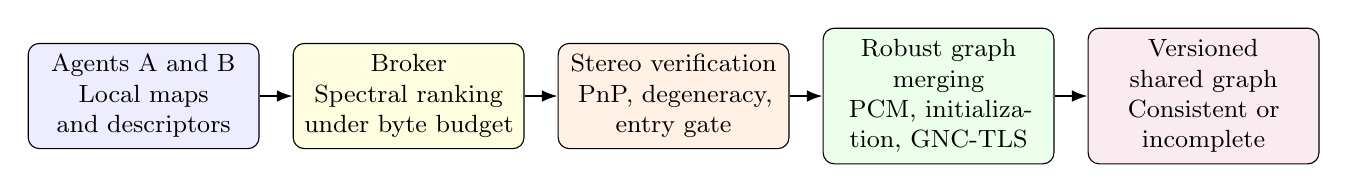
\begin{tikzpicture}[
    node distance=0.42cm and 0.42cm,
    >=Latex,
    stage/.style={
        draw,
        rounded corners,
        align=center,
        text width=2.65cm,
        minimum height=1.05cm,
        font=\small,
        inner sep=4pt
    },
    link/.style={-{Latex[length=2mm]}, thick}
]
\node[stage,fill=blue!7] (agents)
    {Agents A and B\\Local maps and descriptors};

\node[stage,fill=yellow!12,right=of agents] (select)
    {Broker\\Spectral ranking under byte budget};

\node[stage,fill=orange!10,right=of select] (verify)
    {Stereo verification\\PnP, degeneracy, entry gate};

\node[stage,fill=green!8,right=of verify] (robust)
    {Robust graph merging\\PCM, initialization, GNC-TLS};

\node[stage,fill=purple!8,right=of robust] (map)
    {Versioned shared graph\\Consistent or incomplete};

\draw[link] (agents) -- (select);
\draw[link] (select) -- (verify);
\draw[link] (verify) -- (robust);
\draw[link] (robust) -- (map);
\end{tikzpicture}%
}
\caption{Ariadne's collaborative mapping path. Compact descriptors identify
candidate overlaps; budgeted feature exchanges provide geometric evidence;
robust estimation determines which connections enter the shared graph.
The evaluated configuration uses a brokered solve with explicit incomplete
states during communication loss.}
\label{fig:collab-map}
\end{figure*}

\indentedheading{Geometric verification and robust graph merging}

A retrieved match must first survive stereo relative-pose estimation and PnP
verification. Ariadne examines pose covariance, translation and rotation
marginals, parallax, and the spatial distribution of supporting 3D points.
Poorly constrained hypotheses, including nearly collinear correspondences,
are rejected before they can influence graph consistency.

For missions with known relative agent starts, the entry briefing provides
an additional geometric constraint. Each candidate's visual transform is
compared with the transform predicted from the entry prior and accumulated
agent odometry. Covariances are propagated and transported into a common
tangent frame, producing a six-dimensional innovation gate:

\begin{equation}
    r_e =
    \operatorname{Log}\!
    \left(
        (\hat T_e^{\mathrm{prior}})^{-1}
        T_e^{\mathrm{visual}}
    \right),
    \qquad
    r_e^\top\Sigma_e^{-1}r_e
    \leq \chi^2_6(0.999).
    \label{eq:collab-entry-gate}
\end{equation}

Here $\Sigma_e$ includes the relevant prior, odometric, and visual
uncertainties after propagation. The gate exploits information available at
deployment and is enabled only for the evaluated known-start condition.
Unknown relative starts remain vulnerable to perceptual aliasing.

Surviving hypotheses enter pairwise consistency maximization (PCM). Two
closures are compatible when their composition with the intervening
odometry-only paths yields a sufficiently small cycle residual. A consistency
graph records these relationships, and a deterministic greedy clique heuristic
selects mutually supported constraints; exact clique search is available for
small instances. PCM removes isolated false closures efficiently, although a
self-consistent cluster of incorrect matches can survive
\cite{mangelson2018pcm}.

The selected constraints initialize a shared $SE(3)$ pose graph. Without an
entry prior, sparse chordal least squares estimates rotations, projection onto
$SO(3)$ restores valid rotation matrices, and a translation Laplacian supplies
the remaining initialization. With known starts, the entry transforms anchor
the agent frames before joint refinement. Ariadne then applies graduated
non-convexity with truncated least squares (GNC-TLS), progressively adjusting
loop-edge weights according to their whitened residuals while retaining
quadratic odometry factors. This layered backend draws on PCM, robust pose-graph
estimation, and the GNC formulation~\cite{tian2022kimeramulti,yang2020gnc}.

\begin{quote}\small
\textbf{Collaborative update.}
Broadcast compact descriptors; retrieve overlaps and prioritize candidate
exchanges by spectral gain per marginal byte. Request cached feature payloads,
verify stereo geometry and PnP, and reject degenerate hypotheses. Apply the
known-entry Mahalanobis gate when its prior is available. Construct pairwise
consistency relationships, select PCM-compatible closures, initialize the
joint graph, and refine with GNC-TLS. Publish the resulting graph with an
epoch, version, and completeness state.
\end{quote}

\indentedheading{Asynchronous communication and implementation}

A deterministic priority rule elects a broker within each connected
neighborhood. Epochs distinguish broker membership across partitions;
store-and-forward queues preserve messages during disconnection, while
acknowledgements and selective fragment retransmission protect graph data.
On reconnection, agents reconcile graph snapshots under the current epoch.
Missing keyframes or edges leave the shared graph marked incomplete until
their dependencies arrive. This sparse exchange architecture follows the
collaborative principles of Swarm-SLAM, with brokered optimization and
versioned recovery in Ariadne~\cite{lajoie2024swarmslam}.

Wire costs are recorded at the serialization boundary, including framing and
compression. Cached feature payloads and precomputed odometry compositions
reduce repeated matching and PCM work; agents exchange compact graph state
instead of image histories. OpenCV 5 supplies stereo geometry, learned
matching, PnP, and rotation-matrix primitives. Ariadne implements the
protocol, epoch handling, byte ledger, spectral selection, PCM, chordal
initialization, and GNC-TLS backend, using Eigen for sparse spectral and
linear-algebra operations.

\indentedheading{Experimental results}

The most consequential result concerns false map merges. In scene~0, the
ungated configuration produced worst seed-mean merged ATE of
$3.78$--$3.79$\,m across four policy--budget cells. Enabling the known-entry
gate reduced this to \textbf{$0.014675$\,m}; the worst individual gated run
reached $0.0212$\,m. Across both scenes, the gate retained all
\textbf{$560/560$ tested true edges}. Ten additional scene-0 true edges
were never tested by the gate and are excluded from this retention result.
The improvement reflects the combined gated configuration, including its
effect on graph initialization.

Communication selection was evaluated independently on $60$ small synthetic
instances with exact optima. Spectral selection achieved mean
selected-to-optimum utility of \textbf{$0.970$}, against $0.936$ for greedy;
worst-case observed ratios were $0.650$ and $0.533$. These finite-instance
results establish the quality of the implemented heuristic without implying
an approximation guarantee. In the gated simulator sweep, spectral selection
matched or improved greedy in three of four cells, with ATE differences below
approximately $1$\,mm; the fourth cell slightly favored greedy.

In scene~1, budgeted exchange consumed $2.27$--$2.45$\,MB of
first-transmission traffic and yielded $6.8$--$8.6$\,mm merged ATE across
three seeds. The request-everything similarity configuration consumed
$14.8$--$16.0$\,MB; one seed suffered $3.09$\,m aliasing error, while two
runs failed to report a complete multi-agent merge. The configurations
also differ in entry-gate use, so their separation in accuracy cannot be
attributed to communication selection alone.

Byte prediction proved less reliable than the serializer ledger.
All $24$ budgeted request rows met the $15\%$ prediction-error threshold,
with a worst error of $10.65\%$. Response estimates exceeded that threshold
in $8/24$ rows, leaving the overall class-total accounting gate unmet.
Actual transmitted bytes remain measured independently of those estimates.

Controlled robust-backend tests retained all ten planted true inter-agent
loops and rejected every injected false loop across five seeds. PCM followed
by GNC-TLS survived the tested outlier ramp through $90\%$ false loops
in groups of ten, and through $70\%$ with two growing false clusters.
GNC alone also handled the tested ramp at approximately ten times the
runtime. The differing breakpoints expose the dependence of PCM on the
structure of mutually consistent false hypotheses.

\begin{figure*}[t]
  \centering
  \begin{tikzpicture}
    \begin{axis}[name=chi, width=0.5\textwidth, height=4.6cm, xmode=log, xmin=1e-3, xmax=3e4,
        ymin=-0.6, ymax=1.6, ytick={0,1}, yticklabels={false loop, true loop}, xlabel={$d^2=r^\top\Sigma^{-1}r$},
        title={\small (a) known-entry test, logged simulation sweep}, title style={yshift=-1ex},
        tick label style={font=\scriptsize}, label style={font=\scriptsize}]
      \addplot[only marks, mark=*, mark size=0.6pt, red!70!black, opacity=0.5]
        table[x=d2, y=jitter, restrict expr to domain={\thisrow{true}}{0:0}] {figures/data/chi2_separation.csv};
      \addplot[only marks, mark=*, mark size=0.6pt, green!50!black, opacity=0.5]
        table[x=d2, y=jitter, restrict expr to domain={\thisrow{true}}{1:1}] {figures/data/chi2_separation.csv};
      \draw[thick, dashed] (axis cs:22.46,-0.6) -- (axis cs:22.46,1.6) node[pos=0.5, right, font=\scriptsize, fill=white, inner sep=1pt] {cut $\chi^2_6(0.999)=22.46$};
    \end{axis}
    \begin{axis}[at={(chi.east)}, anchor=west, xshift=1.4cm, width=0.5\textwidth, height=4.6cm, ymode=log,
        xmin=0, xmax=60, ymin=0.01, ymax=40, xlabel={mission time (s)}, ylabel={position error (m)},
        title={\small (b) recorded run with the gate off}, title style={yshift=-1ex},
        legend style={font=\scriptsize, at={(0.02,0.98)}, anchor=north west}, tick label style={font=\scriptsize},
        label style={font=\scriptsize}]
      \addplot[blue, thick] table[x=t, y=a0] {figures/data/collab60d_err.csv};
      \addplot[orange, thick] table[x=t, y=a1] {figures/data/collab60d_err.csv};
      \addplot[green!50!black, thick] table[x=t, y=a2] {figures/data/collab60d_err.csv};
      \draw[gray, dashed] (axis cs:40,0.01) -- (axis cs:40,40) node[pos=0.55, left, font=\scriptsize] {false merge};
      \legend{robot 1, robot 2, robot 3}
    \end{axis}
  \end{tikzpicture}
  \caption{Why the known-entry gate exists. (a) Every geometry-verified inter-agent candidate in the logged sweep
  (\code{evaluation/runs/collab\_d178/logged\_4ec3f6}): 560 true loops (pose error $\le 10^\circ$) score
  $d^2\le 1.1$, 1{,}164 false loops score $d^2\ge 6{,}175$, against a 22.46 cut. (b) A recorded three-robot run with
  the gate off (\code{collab60d}): 32 of 491 candidates pass every geometric check, all 32 are false, and a false
  merge at $t=40$\,s leaves robot~2 15.3\,m off. In a second recorded run with the gate on, it refused 8 of 8
  tested candidates and every robot stayed within 7.5\,cm of ground truth. Data: \code{figures/data/*.csv}, derived by
  \code{figures/src/make\_stills.py}.}
  \label{fig:gate}
\end{figure*}

\indentedheading{Comparison with prior systems}

\begin{table*}[t]
\centering
\small
\setlength{\tabcolsep}{5pt}
\begin{tabular}{@{}
    p{0.19\textwidth}
    p{0.33\textwidth}
    p{0.42\textwidth}
@{}}
\toprule
\textbf{Aspect} &
\textbf{Ariadne evidence} &
\textbf{Relationship to prior work} \\
\midrule

Budgeted exchange &
$0.970$ mean spectral utility ratio against exact optima
on $60$ synthetic instances. &
Tian et al.\ establish task-oriented exchange;
Ariadne evaluates Laplacian connectivity against measured
serialization costs~\cite{tian2018near}. \\

Robust merging &
$560/560$ tested true edges retained by the known-entry
gate; scene-0 worst seed-mean ATE reduced to $1.47$\,cm. &
PCM and Kimera-Multi motivate consistency-based rejection
and robust optimization. Ariadne adds a deployment-specific
entry prior, evaluated without a common-dataset comparison
\cite{mangelson2018pcm,tian2022kimeramulti}. \\

Communication protocol &
Broker epochs, selective retransmission, store-and-forward,
and explicit incomplete graph states. &
Swarm-SLAM motivates sparse collaborative exchange;
Ariadne uses a versioned brokered solve with replayable
partition recovery~\cite{lajoie2024swarmslam}. \\

\bottomrule
\end{tabular}
\caption{Architectural and algorithmic comparison. Reported Ariadne
measurements come from its own synthetic and simulated evaluations;
the cited systems use different experimental settings.}
\label{tab:collab-prior-work}
\end{table*}

Together, these experiments identify the condition under which sparse
collaboration becomes dependable. Communication-aware selection substantially
reduces transmitted evidence, while geometric verification, the entry prior,
PCM, and GNC-TLS limit the damage caused by ambiguous visual matches.
Known-start scenes demonstrate a reliable shared graph at low communication
cost; unknown-start aliasing and imperfect byte prediction remain measured
limits of the approach.


\section{Exploration, mapping, and task allocation}

Ariadne closes the loop between observing a space and deciding where to look
next. Stereo depth and estimated poses accumulate into a volumetric map;
uncertainty, clearance, and connectivity then guide candidate views and
multi-agent task allocation. The same geometry supports a second decision:
whether a responder can reach a validated exit from a location of interest.
Exploration seeks useful observations under mission constraints, while egress
planning depends on observed, body-sized passages.

\begin{figure*}[t]
\centering
\resizebox{\linewidth}{!}{%
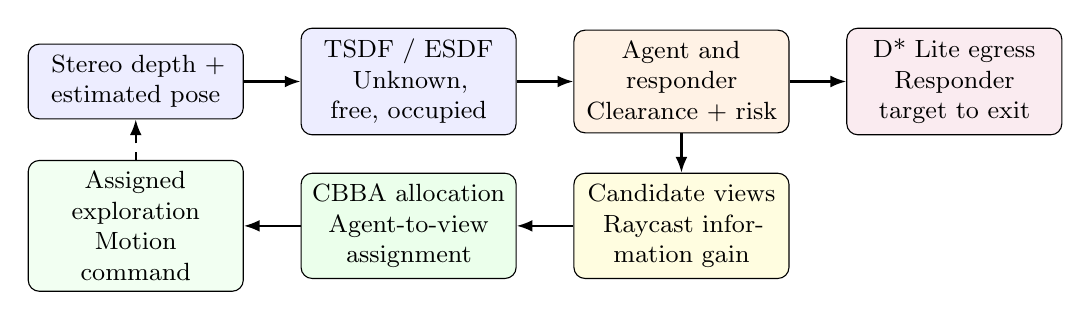
\begin{tikzpicture}[
    node distance=0.50cm and 0.72cm,
    >=Latex,
    box/.style={
        draw,
        rounded corners,
        align=center,
        text width=2.45cm,
        minimum height=0.72cm,
        font=\small,
        inner sep=4pt
    },
    link/.style={-{Latex[length=2mm]},thick}
]
\node[box,fill=blue!7] (depth)
    {Stereo depth + estimated pose};

\node[box,fill=blue!7,right=of depth] (map)
    {TSDF / ESDF\\Unknown, free, occupied};

\node[box,fill=orange!10,right=of map] (trav)
    {Agent and responder\\Clearance + risk};

\node[box,fill=purple!8,right=of trav] (route)
    {D* Lite egress\\Responder target to exit};

\node[box,fill=yellow!12,below=of trav] (views)
    {Candidate views\\Raycast information gain};

\node[box,fill=green!8,left=of views] (auction)
    {CBBA allocation\\Agent-to-view assignment};

\node[box,fill=green!5,left=of auction] (motion)
    {Assigned exploration\\Motion command};

\draw[link] (depth) -- (map);
\draw[link] (map) -- (trav);
\draw[link] (trav) -- (route);
\draw[link] (trav) -- (views);
\draw[link] (views) -- (auction);
\draw[link] (auction) -- (motion);
\draw[link,dashed] (motion.north) -- (depth.south);
\end{tikzpicture}%
}
\caption{The map-to-action loop. Exploration assigns informative views to
agents and incorporates their subsequent observations; responder-scale egress
planning branches from the same volumetric model.}
\label{fig:planning-loop}
\end{figure*}

\indentedheading{Volumetric map and compute path}

Stereo observations enter a $5$\,cm voxel-hash truncated signed distance
field (TSDF), organized into $8^3$-voxel blocks. Each voxel stores a signed
distance $D_v$ and accumulated confidence weight $W_v$, updated by
uncertainty-weighted ray integration within a three-voxel truncation band.
A zero weight preserves the unknown state, distinguishing unobserved space
from measured free space. The map maintains separate Euclidean signed
distance fields (ESDFs): agent planning treats occupied cells as obstacles,
while responder planning additionally excludes unknown cells. Exact
one-dimensional squared-distance transforms along each voxel axis recover
3D Euclidean clearance, with incremental recomputation around changed
regions. A $0.5$\,m coarse layer and maintained frontier clusters support
longer-range exploration.

Resolution follows the geometry of the intended user. At $8$ and $10$\,cm,
one-cell wall bleed closed a $1.05$\,m entrance to a $0.40$\,m-radius
responder in both tested ground-truth scenes; $5$\,cm preserved the passage.
Against Ariadne's earlier OctoMap-based placeholder on the same evidence
spool, TSDF coverage improved from $0.933$ to \textbf{$0.942$},
free-space precision from $0.961$ to $0.979$, and occupied-space precision
from $0.707$ to \textbf{$0.865$}. Mean per-keyframe integration cost was
$16.1$\,ms; incremental ESDF and frontier updates averaged $64.3$ and
$48.3$\,ms on the development host.

The block-hash fusion and frontier-update designs draw on Voxblox and
FUEL~\cite{voxblox2017,fuel2021}. Ariadne implements voxel storage,
weighted fusion, distance queries, and incremental updates because the
required per-voxel access is absent from the evaluated OpenCV volume
interface, while OpenCV's distance transform operates in 2D.
\code{cv::PCA} partitions large frontier clusters,
\code{cv::filter2D} computes local support statistics, and
\code{cv::parallel_for\_} distributes candidate scoring.
The earlier occupancy baseline uses an OctoMap-style
representation~\cite{octomap2013}.

\indentedheading{Body-aware traversability and structural-risk proxy}

Responder clearance requires a different interpretation of unknown
geometry. A strict observed-volume test would reject much of a standing
body above a camera operating near $1$\,m height. Ariadne combines a
$2.5$D ground lattice with 3D capsule collision checks, requiring
observed ground support, sufficient planar clearance, and unobstructed
body geometry. The evaluated responder has radius $0.40$\,m and height
$1.80$\,m; agents use their own capsule and altitude constraints.

Evaluation covers every ground-truth-labelled cell of the aligned ground
grid, including $12{,}334$ traversable cells. Unknown predictions count
against recall, and any claimed passage through a ground-truth obstacle
counts against precision. The hybrid test achieved
\textbf{$1.000$ precision and $0.900$ recall}, with no false traversability
claims and valid connections from both tested starts to the target.
Strict 3D observed-volume clearance achieved the same precision but only
$0.354$ recall, closing both routes; unobserved voxels caused $91\%$
of its missed traversable cells. The earlier placeholder reached
$0.898$ recall. These results describe the evaluated ground-plane grid
and its observation geometry.

A separate structural-risk proxy estimates overhanging occupied mass and
poorly supported surfaces above an otherwise open walking column:

\begin{equation}
    r =
    1-(1-r_{\mathrm{overhang}})
      (1-r_{\mathrm{unsupported}}).
    \label{eq:structural-risk}
\end{equation}

Against procedural hazard labels, the combined proxy achieved ROC AUC
\textbf{$0.831$}, exceeding the preregistered $0.75$ threshold.
Its operating threshold nevertheless saturated at $1.0$, producing a
$0.338$ false-positive rate in traversable cells outside labelled zones.
The overhang term alone reached $0.922$ AUC with $0.156$ false-positive
rate, but remains an unelected alternative.

Risk enters the route objective, so calibration affects the route itself.
In one hazard seed, risk-weighted planning avoided the labelled zone at
unchanged path length ($4.991$\,m), reducing estimated route risk from
$0.340$ to zero. In another, an already safe route lengthened by $4.4\%$
without reducing estimated risk. The proxy therefore supplies a measurable
geometric warning signal, with false positives that can impose unnecessary
detours. It does not establish structural integrity or predict collapse.

\begin{figure}[t]
  \centering
  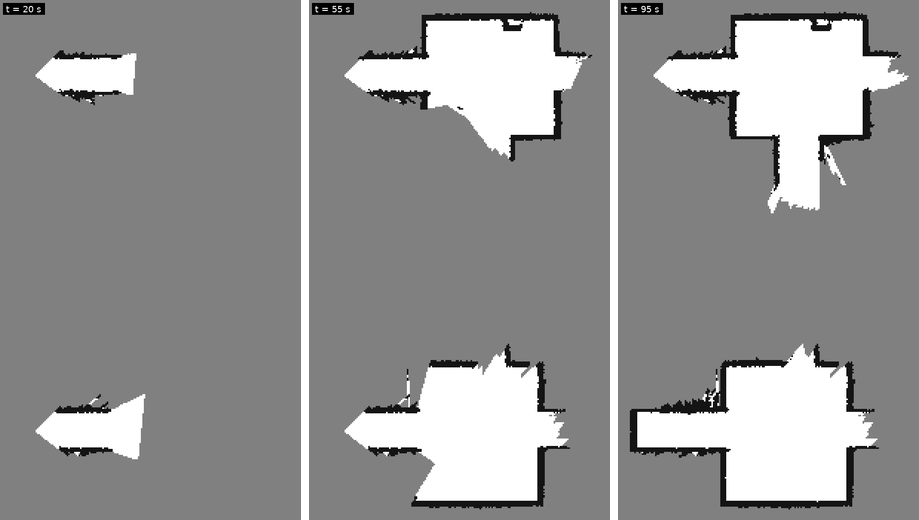
\includegraphics[width=\linewidth]{fig_slabs.png}
  \caption{The volumetric map growing during the final-stack recorded run (two agents, \code{maze\_short\_6},
  200\,s, AWS). Occupancy slab of the Phase-4 TSDF/ESDF map at three times: white is observed free space, black
  is surface, grey is unknown.}
  \label{fig:slabs}
\end{figure}

\indentedheading{Next-best-view planning}

Each map update can expose new frontiers, weakly observed coarse cells,
unrevisited peer keyframes, suspected place aliases, or poorly supported
egress segments. These five sources generate candidate observations.
A cylindrical sampler places viewpoints at radii $1.0$, $1.5$, and
$2.0$\,m, across $16$ azimuths at $1.0$\,m height. Collision and
line-of-sight tests remove infeasible views; two viewpoints per target
advance to detailed scoring.

Ariadne estimates expected information gain by raycasting candidate
camera frusta into the volumetric map. A $64$-ray pass ranks views by
coverage, followed by $256$ rays over a $2.84$\,m depth horizon for the
retained candidates. Voxels are deduplicated within each frustum.
The utility combines expected coverage, entropy reduction, egress
support, graph-connectivity improvement, and alias disambiguation:

\begin{align}
G(a) ={}&
    \widehat{\Delta C}(a)
  + \widehat{\Delta H}(a)
  + \widehat{\Delta E}(a)
  + \widehat{\Delta P}(a)
  + \widehat{\Delta L}(a),
    \label{eq:nbv-gain}\\
U(a) ={}&
    G(a)
  - \lambda_{\mathrm{path}}(t)C_{\mathrm{path}}(a)
  - C_{\mathrm{bandwidth}}(a)
  - C_{\mathrm{risk}}(a).
    \label{eq:nbv-utility}
\end{align}

Each gain term is normalized by its current candidate-set $90$th
percentile, falling back to its maximum when necessary; an identically
zero term contributes zero. Observation-weight entropy rewards poorly
constrained surfaces even after their first sighting. Terms lacking
a producer in the evaluated configuration remain zero. The path-cost
weight increases with mission time and energy expenditure, while a
hard reserve rule restricts proposals to return or hold whenever
remaining energy falls below $1.3$ times the estimated safe-return
requirement. Independent targets are evaluated in parallel.

The preregistered coverage-versus-time hypothesis failed. Across
$36$ closed-loop runs spanning two scenes, six policies, and three seeds,
Ariadne ranked third by coverage AUC in both scenes: $0.884$ on
\code{ci\_tiny} and $0.440$ on \code{maze\_short}, against
$0.892$/$0.495$ for coverage-greedy and $0.895$/$0.443$ for the
TARE-inspired policy. Ariadne eventually led all six policies on
\code{ci\_tiny} after $80$\,s and attained the highest
\code{maze\_short} coverage at $200$\,s ($0.757$, versus $0.713$
and $0.681$). Its slower initial progress nevertheless reduced
area under the coverage-time curve.

Execution traces help explain the gap. Agents spent $45$--$46\%$
of mission time rotating and $31$--$32\%$ translating. Approximately
half the turning arose from heading reversals between approaching a
viewpoint and facing its observation target. An arrival-heading option
and time-aware command cost have been implemented, alongside fixes for
at-cell views and cut commands; the time-aware variant has yet to
complete the full evaluation. The measured comparison therefore
retains the original path-cost policy.

The TARE-inspired comparator schedules coarse $6$\,m subspaces and
constructs local tours through nearest-neighbour insertion and 2-opt
refinement~\cite{tare2021}. On $200$ synthetic tours of at most eight
nodes, its worst score was $0.811$ of exact enumeration. Its simulator
results characterize this adapted policy rather than the published
TARE system.

\indentedheading{Multi-agent task allocation}

Candidate views become stable tasks shared between agents. Ariadne
uses event-triggered Consensus-Based Bundle Algorithm (CBBA) with
bundle length $L_t=1$. Each agent computes the value of an ordered
task bundle $p$ using a time-discounted, diminishing-gain score:

\begin{equation}
    S_i(p)=
    \sum_{j\in p}
    \bar c_{ij}
    \exp\!\left(
        -\frac{\lambda_{\mathrm{path}}
               d_{ij}(p)}
              {P_{\mathrm{path}}}
    \right),
    \label{eq:cbba-score}
\end{equation}

where $\bar c_{ij}$ incorporates task information value after bandwidth
and risk costs, $d_{ij}(p)$ is geodesic travel distance within the
ordered bundle, and $P_{\mathrm{path}}$ is a shared scale frozen for
each auction event. Agents exchange winner, bid, and timestamp state
when tasks appear, complete, or communication topology changes.
Sparse consensus messages carry only tasks with assigned winners.
A broker-side sequential greedy allocator (SGA) uses identical scores
and tie-breaking as a reference. The score is designed for CBBA's
diminishing-marginal-gain assumptions; its published convergence
conditions additionally depend on communication and consensus
behavior~\cite{cbba}.

Across $40$ two-agent replay replans, CBBA and SGA agreed on every
assignment. For the $12$ linked replans permitting exact enumeration,
CBBA reached mean \textbf{$0.994$} of optimum, with worst ratio
$0.983$. Sparse consensus messages averaged $226$ bytes and consumed
$11.8$\,kB overall, compared with $123.4$\,kB for dense exchange.
Partition behavior was exercised in synthetic tests; the replay
establishes agreement and byte savings under its evaluated two-agent
connectivity conditions.

\section{Safe egress planning and replanning}

Ariadne's egress planner turns the shared map into a route a responder
could follow home. Given a location of interest and validated exits,
it searches for a connected passage with sufficient body clearance
and observational support. Routes occupy a 2D ground lattice, with
3D collision checks against the responder ESDF. Unknown or blocked
columns are excluded from the graph, so uncertainty penalties can
favor better-observed passages without admitting unverified ones.

\indentedheading{Route graph and cost}

The lattice is 8-connected, with diagonal moves constrained by
corner occupancy. Each node represents a responder-traversable
column, and each legal edge $x\rightarrow y$ carries a cost

\begin{equation}
\begin{aligned}
c(x,y) = \|x-y\|\Bigg[
    1
    &+ w_u(1-s_{xy})
    + w_r r_{xy} \\
    &+ w_c
    \frac{\max(0,\rho_{\mathrm{safe}}-d_{xy})}
         {\rho_{\mathrm{safe}}}
\Bigg],
\end{aligned}
\label{eq:egress-cost}
\end{equation}

where $s_{xy}$ is observed support over the responder-body envelope,
$r_{xy}$ is the structural-risk proxy, and $d_{xy}$ is ESDF
clearance. Nonnegative penalties ensure $c(x,y)\geq\|x-y\|$,
preserving the consistency of the octile-distance heuristic.
Cost weights were fixed before evaluation. The main egress spool
used $w_r=0$; risk-weighted routing was evaluated separately after
the proxy passed its preregistered calibration threshold.

Route confidence is the fifth percentile of support along the
selected path, exposing short, poorly observed stretches that a
mean would conceal. It summarizes geometric observation support;
calibration against real traversal outcomes remains outside the
evaluation.

\indentedheading{Incremental multi-exit search}

Ariadne uses multi-source D* Lite, propagating cost-to-exit backward
from every traversable exit. Exit nodes have $\mathrm{rhs}=0$;
other nodes maintain the one-step Bellman estimate

\begin{equation}
\mathrm{rhs}(u)=
\min_{v\in\mathrm{Succ}(u)}
\left[c(u,v)+g(v)\right],
\qquad
\mathrm{key}(u)=
\begin{pmatrix}
\min(g,\mathrm{rhs})+h(u,s)\\
\min(g,\mathrm{rhs})
\end{pmatrix},
\label{eq:egress-dstar}
\end{equation}

where $s$ is the fixed responder target and $h$ is octile distance.
Only locally inconsistent vertices, $g(u)\neq\mathrm{rhs}(u)$,
enter the priority queue. Once the target is consistent, the route
follows successive legal neighbors minimizing $c(u,v)+g(v)$.

Changes to occupancy, clearance, or support invalidate affected
edges and trigger repairs to their incident vertices. Ariadne
updates each changed cell's $3\times3$ neighborhood because diagonal
corner legality also depends on adjacent orthogonal cells.
The search reuses unaffected cost-to-go estimates, with no
moving-start correction for the fixed target~\cite{dstar2002}.
Tests exercise multiple exits, blocked corners, and doorway
closure after route construction.

\indentedheading{Evaluation and replanning}

Across $180$ randomized occupancy and edge-cost updates, incremental
D* Lite reproduced fresh multi-source Dijkstra solutions exactly.
It expanded \textbf{$17{,}564$ vertices}, against $132{,}932$
for repeated fresh searches, a $7.6\times$ reduction.

On the recorded mission spool, all \textbf{$12/12$ routes} were
ground-truth traversable. The final $4.44142$\,m route agreed with
the $4.4414215$\,m ground-truth geodesic, and the first valid route
appeared at $145$\,s. Incremental search nevertheless averaged
$0.46$\,ms per query against $0.04$\,ms for fresh A* on this short,
nearly straight problem. End-to-end replanning averaged $545$\,ms
(p95 $651$\,ms), including support and traversability updates.
The available profile does not isolate their individual costs.

The mission spool contained no obstruction discovered directly
on an active route. A separate doorway-closure test verified path
replacement or explicit no-path reporting. Thus, the mission
establishes route validity and repeated map-to-route operation;
the controlled test establishes response to route invalidation.

Risk-aware routing exposed the cost of imperfect calibration.
In one hazard seed, the planner avoided the labelled hazard
without increasing its $4.991$\,m path length, reducing estimated
risk from $0.340$ to zero. In another, saturation of the risk
proxy lengthened an already hazard-free route by $4.4\%$, with no
reduction in estimated risk. Geometric risk can therefore improve
route choice, but false positives can also impose unnecessary
detours.

\indentedheading{Visibility-graph alternative}

A FAR-inspired dynamic visibility graph was evaluated as a
lightweight alternative. On $12$ short-spool queries, its
string-pulled route matched the lattice result at $4.403$\,m;
graphs contained at most $31$ nodes, with mean update and query
times of $0.7$ and $0.01$\,ms. A later hazard case exposed a
missed passage: the visibility graph returned $11.115$\,m against
a $4.424$\,m lattice route. This counterexample prevents a
general path-quality claim for the implemented graph.

FAR motivates efficient visibility-graph maintenance and permits
exploratory routes through unknown regions~\cite{far2022}.
Ariadne retains the conservative lattice for reported responder
egress, where every route segment must satisfy known-space
traversability.

\indentedheading{OpenCV 5 boundary}

The volumetric clearance and incremental search algorithms are
Ariadne implementations. OpenCV 5 supplies adjacent geometric
operations: \code{cv::filter2D} for support and risk aggregation,
\code{cv::findContours} and \code{cv::approxPolyDP} for experimental
visibility-graph construction, and the upstream stereo-depth
primitives. TSDF fusion, 3D ESDF maintenance, route costs, and
D* Lite remain explicit components of the planning system.



\section{Language-model task decisions and human authority}

Ariadne's language-model layer enters where the geometric planner has
already identified useful actions. At each replan, the deterministic
mission layer constructs feasible observation tasks from the current
map, agent poses, uncertainty, and resource estimates. A multimodal
model examines this bounded decision context and selects among the
proposals. Its choices pass through runtime validation before becoming
motion commands, keeping geometric feasibility, collision checks,
and responder egress within the established planning system.

\indentedheading{Decision architecture and authority}

The orchestrator receives one joint decision request per replan,
containing candidate tasks, agent assignments, route summaries,
uncertainty, and a compact visual map. It returns candidate indices
with a short rationale and may propose directives to prioritize or
exclude regions, assign tasks, or hold agents. Directives require
operator confirmation and take effect at a subsequent planning
boundary. Candidate validation checks membership, feasibility,
risk, and assignment uniqueness before dispatch.

\begin{figure*}[t]
\centering
\resizebox{0.94\textwidth}{!}{%
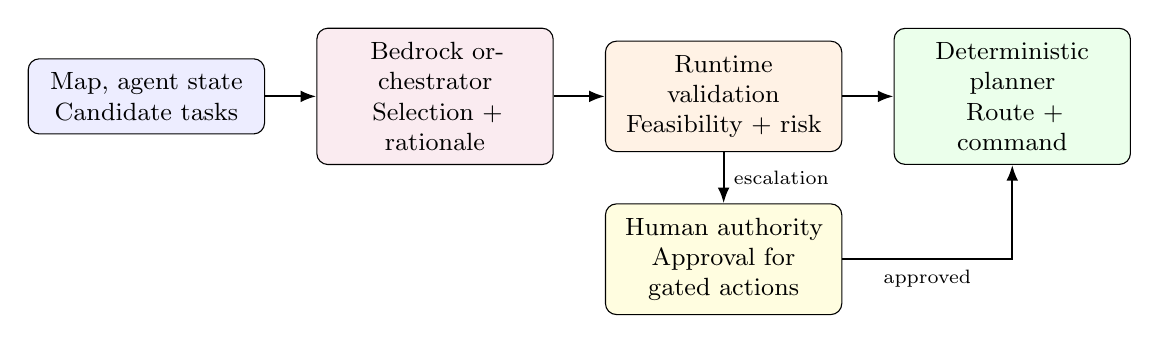
\begin{tikzpicture}[
    node distance=0.55cm and 0.65cm,
    >=Latex,
    box/.style={
        draw,
        rounded corners,
        align=center,
        text width=2.65cm,
        minimum height=0.88cm,
        font=\small,
        inner sep=5pt
    },
    link/.style={-{Latex[length=2mm]},thick}
]
\node[box,fill=blue!7] (state)
    {Map, agent state\\Candidate tasks};

\node[box,fill=purple!8,right=of state] (model)
    {Bedrock orchestrator\\Selection + rationale};

\node[box,fill=orange!10,right=of model] (validate)
    {Runtime validation\\Feasibility + risk};

\node[box,fill=green!8,right=of validate] (dispatch)
    {Deterministic planner\\Route + command};

\node[box,fill=yellow!12,below=0.65cm of validate] (human)
    {Human authority\\Approval for gated actions};

\draw[link] (state) -- (model);
\draw[link] (model) -- (validate);
\draw[link] (validate) -- (dispatch);
\draw[link] (validate) --
    node[right,font=\scriptsize]{escalation} (human);
\draw[link] (human.east) -|
    node[pos=0.25,below,font=\scriptsize]{approved}
    (dispatch.south);

\end{tikzpicture}%
}
\caption{Task-level orchestration and intended authority boundary.
The model selects planner-generated candidates; runtime validation
and, where required, human approval precede deterministic dispatch.
The separate egress planner computes responder routes directly
from the geometric map.}
\label{fig:llm-control}
\end{figure*}

Exploration decisions return to the sensing loop as movement produces
new observations and changes the next candidate set. Responder egress
remains an independent map query, allowing a validated exit route to
be computed regardless of the model's exploration choice.

\indentedheading{Runtime, tools, and approval}

The orchestration service exposes image, map, uncertainty, route,
and candidate queries through the Model Context Protocol (MCP).
Amazon Bedrock Converse invokes Nova 2 Lite for multimodal selection;
a configured DeepSeek text model provides a provider-error fallback.
A browser-based demonstration console presents live map and agent
state, planning decisions, and operator controls, while the service
layer manages model calls and tool responses. Request and response
payloads, tool calls, candidate selections, directives, and state
digests are recorded for deterministic replay. Replay reproduces
the recorded decisions; fresh model inference remains stochastic.

Actions requiring review are identified by a heuristic combining
clearance and estimated structural risk:

\begin{equation}
\begin{aligned}
r &= \max(r_{\mathrm{geom}},r_{\mathrm{structural}}),\\
r_{\mathrm{geom}} &=
\operatorname{clamp}\!\left(
\frac{\rho_{\mathrm{responder}}-c_{\min}}
{\rho_{\mathrm{responder}}-\rho_{\mathrm{agent}}},
0,1\right).
\end{aligned}
\label{eq:agentic-risk}
\end{equation}

Here $c_{\min}$ is estimated clearance and
$r_{\mathrm{structural}}$ is the geometric risk proxy.
The approval threshold, fixed at $0.5$, is a policy parameter
on this normalized score. The formula requires finite clearance
and $\rho_{\mathrm{responder}}>\rho_{\mathrm{agent}}>0$.
Startup configuration does not yet enforce this domain,
leaving a validation defect in the gate.

The model-choice validator, approval request, and rejection paths
are implemented and exercised in scripted and Bedrock-stub tests.
Live runs remained below the threshold, leaving operator approval,
rejection, and timeout unexercised with a real model. Code review
also exposed a dispatch defect: after rejection, the original
joint allocation can remain scheduled despite a fallback label.
The computed risk-filtered alternative is not consistently
substituted and revalidated. Consequently, the intended approval
boundary is implemented only partially, and the live evidence
does not establish rejection-safe dispatch. Duplicate assignments
are checked within each joint decision; execution across retries
and failures has no exactly-once guarantee.

\indentedheading{Live evaluation and reproducibility}

An initial two-agent, $90$-second mission in
\code{maze\_short\_6} completed $18$ joint replans and
\textbf{$36/36$ Nova 2 Lite assignments}, without model errors,
fallbacks, or runtime crashes. Its two recorded replays passed
all $15$ checks covering inputs, estimator state, directives,
movement, and trace hashes. The initial artifact carried a
dirty-tree and configuration-provenance inconsistency, motivating
a matched comparison from a common source revision.

The subsequent classical--Bedrock pair fixed scene, seed,
renderer, runtime, and mission configuration at revision
\code{c143db14}, changing only the chooser. Both arms completed
$18$ joint replans and $36$ agent decisions, with passing replay
verdicts. Bedrock differed from the classical agent-0 choice
on $6/18$ replans and selected rank-zero candidates $31/36$
times, compared with $26/36$ for the classical arm. Each arm
issued $36$ commands, of which $34$ were accepted and two
remained unanswered at termination; none were refused.

A longer matched pair extended the same experiment to
$500$ simulated seconds. Both arms completed $100$ joint
replans, issued $200$ commands, and recorded $10{,}001$
frames per agent without unpaired-frame losses. Two replays
per arm reproduced the live state digests and matched each
other exactly. These experiments establish sustained live
orchestration, behavioral differences between choosers, and
reproducible recorded execution. Ground-truth coverage,
egress validity, and mission completion were not scored
between arms, leaving comparative mission benefit unresolved.

Model inference also carries a measurable operational cost.
Across the $18$ decisions of the matched Bedrock run,
orchestration latency had median $5.8$\,s, p90 $7.45$\,s,
and maximum $9.03$\,s, excluding C++ planning and motion.
The trace recorded $2{,}936{,}424$ input tokens over $118$
Bedrock calls. Tool exchanges repeatedly resubmit context,
so this cumulative count exceeds the unique decision input;
billing reconciliation was not performed. The matched
$90$-second missions required $611$\,s and $616$\,s of wall
time for the classical and Bedrock arms, respectively.
The $500$-second recordings are indexed under
\code{evaluation/runs/agentic\_planning\_pair\_500s\_20261025/}.

\begin{figure}[t]
  \centering
  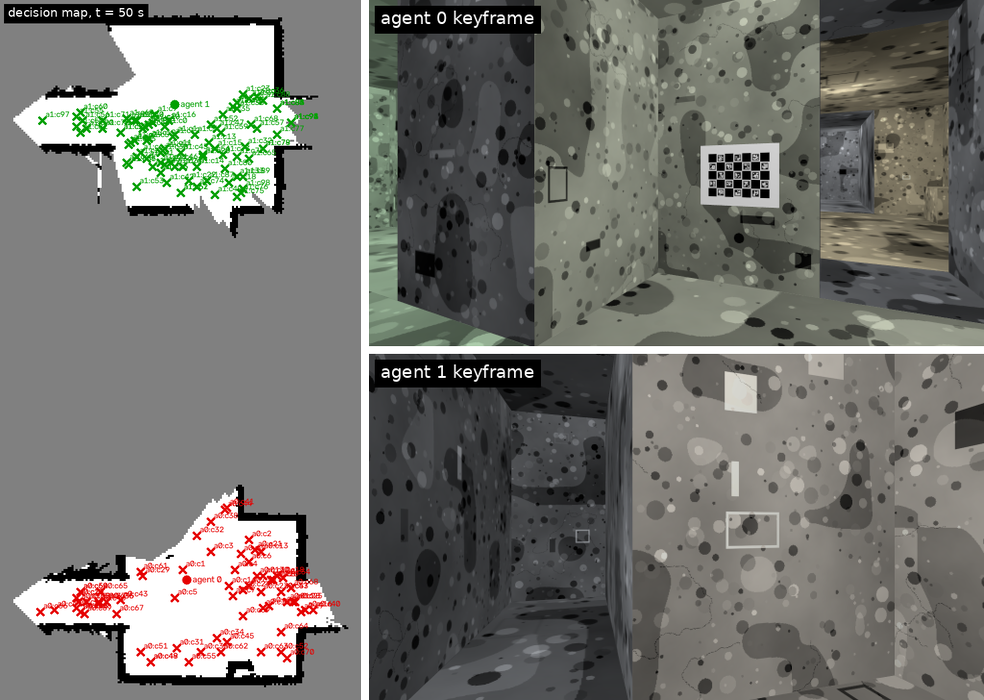
\includegraphics[width=\linewidth]{fig_decision.png}
  \caption{What the orchestrator sees at one decision of the final-stack recorded run ($t=50$\,s): the
  OpenCV-rendered map returned by \code{observe\_image}, with each agent's candidate goals, and the two agents'
  keyframes at that instant. That run made 40 joint replans and 80 Nova~2~Lite decisions, all validated by the
  C++ checks, with a passing replay.}
  \label{fig:decision}
\end{figure}

\indentedheading{Relationship to language-guided navigation}

Language-guided exploration provides useful architectural
precedents. L3MVN and LFG score navigation frontiers using
language-model reasoning; SayNav grounds task plans in scene
graphs and delegates motion to conventional navigation; Co-NavGPT
extends vision-language task assignment to cooperating robots
\cite{l3mvn,lfg,saynav,conavgpt}. Ariadne applies bounded model
selection to candidates generated from geometric uncertainty,
connectivity, communication cost, and risk. Its matched experiments
demonstrate that language-model decisions can alter the exploration
schedule while remaining replayable through the deterministic
runtime. Establishing whether those changes improve completed
missions requires ground-truth outcomes across additional scenes
and seeds, together with a verified approval and fallback path.






\section{Gaussian-splat reconstruction: an inspectable surface model}

Ariadne's Gaussian map gives incident command a view of the explored
space beyond the agents' recorded camera positions. Each Gaussian
encodes a 3D mean, anisotropic scale, orientation, opacity, and colour;
differentiable rasterization projects these primitives into novel
views. The representation complements the geometric map used for
clearance and egress. Reconstruction consumes validated poses and
stereo depths, allowing the visual scene to evolve independently of
localization and route planning.

The service receives rectified RGB, metric depth, depth uncertainty,
and keyframe poses. It initializes Gaussians from stereo observations,
groups them into anchor-relative submaps, optionally refines active
submaps on a GPU, and exports compact chunks to a Spark/WebGL browser
viewer. Training and browser rendering have separate compute budgets.

\begin{figure*}[t]
\centering
\resizebox{0.94\linewidth}{!}{%
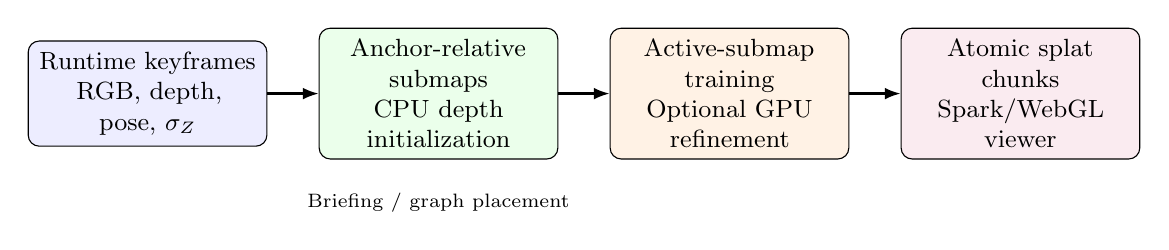
\begin{tikzpicture}[
    node distance=0.45cm and 0.65cm,
    >=Latex,
    box/.style={
        draw,rounded corners,align=center,
        text width=2.75cm,minimum height=0.83cm,
        font=\small,inner sep=4pt
    },
    link/.style={-{Latex[length=2mm]},thick}
]
\node[box,fill=blue!7] (input)
    {Runtime keyframes\\RGB, depth, pose, $\sigma_Z$};

\node[box,fill=green!8,right=of input] (submap)
    {Anchor-relative submaps\\CPU depth initialization};

\node[box,fill=orange!10,right=of submap] (train)
    {Active-submap training\\Optional GPU refinement};

\node[box,fill=purple!8,right=of train] (viewer)
    {Atomic splat chunks\\Spark/WebGL viewer};

\draw[link] (input)--(submap);
\draw[link] (submap)--(train);
\draw[link] (train)--(viewer);

\node[font=\scriptsize,below=3mm of submap]
    {Briefing / graph placement};
\end{tikzpicture}%
}
\caption{Reconstruction from validated stereo keyframes to browser-visible
Gaussian submaps. The live demonstration exercised CPU initialization and
streaming; GPU refinement was evaluated separately.}
\label{fig:splat-pipeline}
\end{figure*}

\indentedheading{Submap frames and live transport}

Each agent maintains submaps in the coordinate frame of an anchor
keyframe. For agent odometry frame $O_k$, submap anchor $A_s$, and
keyframe camera $C$, a depth sample is initialized through

\begin{equation}
\begin{aligned}
T_{A_sC} &= T_{O_kA_s}^{-1}T_{O_kC},
& X_{A_s} &= T_{A_sC}X_C,\\
T_{WA_s} &= T_{WO_k}T_{O_kA_s}.
\end{aligned}
\label{eq:splat-frames}
\end{equation}

Gaussians remain in anchor coordinates. The browser applies
$T_{WA_s}$ once per submap, allowing an updated global placement
to move the entire chunk without rewriting its Gaussian parameters.
Submaps close after $30$ keyframes or at correction boundaries.
Rigid re-anchoring preserves internal Gaussian geometry; corrections
within a submap require further refinement. This bounded-submap
design follows the geometric separation explored by
LoopSplat~\cite{loopsplat}.

A nonblocking runtime tee sends length-prefixed
\texttt{\#kf} records over a local socket, with an eight-keyframe
queue per agent and accounted oldest-first drops. Records contain
agent and keyframe IDs, timestamps, pose versions, camera geometry,
rectified RGB, and half-resolution float16 depth $Z$ and axial
uncertainty $S=\sigma_Z$. Placement records carry $T_{WO_k}$.
The uncertainty follows stereo propagation,

\begin{equation}
    \sigma_Z=\frac{Z^2}{f_xB}\sigma_d,
    \label{eq:splat-depth-uncertainty}
\end{equation}

where $f_x$, $B$, and $\sigma_d$ denote focal length, baseline,
and disparity-error proxy. Pose uncertainty is excluded from
this estimate. The receiver validates payloads, frame conventions,
and agent placement before accepting keyframes.

The service atomically publishes a placement table and one
\texttt{.splat} chunk per submap. Each Gaussian occupies $32$
bytes with degree-zero spherical harmonics; the table carries
chunk identity, anchor, pose version, Gaussian count, and world
transform. Active chunks may be replaced, while closed chunks
remain fixed. Spark 2.3.1 renders one mesh per submap, applying
placement independently of chunk contents.

\indentedheading{Depth seeding and Gaussian refinement}

The initial fused-cloud renderer established the reconstruction
interface but produced soft, incomplete surfaces. Subsequent
experiments adopted a Gaussian-SLAM-style depth-seeding and
joint appearance--geometry objective~\cite{gaussianslam}.
The first keyframe samples valid depth uniformly and from
high-gradient image regions, using fractions
$100000/307200$ and $50000/307200$, respectively.
Later keyframes target pixels whose rendered alpha is below
$0.6$. Samples require $0<Z\leq6$\,m and
$\sigma_Z\leq0.05$\,m; a nearest-neighbour check excludes
points within $1$\,cm of existing active-submap Gaussians.
Accepted points receive local-distance scales, source-image
colours, and initial opacity $0.5$.

The active submap is optimized with gsplat 1.5.3 and PyTorch.
Its adopted objective is

\begin{equation}
\mathcal{L}=
0.8\mathcal{L}_{1,\mathrm{colour}}
+0.2\mathcal{L}_{\mathrm{DSSIM}}
+\mathcal{L}_{1,\mathrm{depth}}
+\mathcal{L}_{\mathrm{isotropy}},
\label{eq:splat-loss}
\end{equation}

where $\mathcal{L}_{\mathrm{DSSIM}}=1-\mathrm{SSIM}$ and
the isotropy regularizer penalizes deviations of each Gaussian
scale axis from its mean. Colour and metric-depth residuals
share a finite-value, uncertainty-thresholded pixel mask;
depth residuals receive no inverse-variance weighting.
At least $40\%$ of iterations sample the newest keyframe,
with remaining iterations drawn from the active submap.
Low-opacity Gaussians are pruned midway and after each update.

A projected Gaussian gains one consistency count per processed
keyframe when its axial depth agrees with the measured depth
within $3\sigma_Z$. After $15$ consistent keyframes it becomes
stable: its parameters are frozen, and Adam moments are cleared
to prevent momentum-driven updates. The threshold translates
RTG-SLAM's temporal support criterion to Ariadne's measured
keyframe rate and remains an uncalibrated design choice
\cite{rtgslam}. Growth uses depth seeding; gradient-driven
clone/split densification and cross-agent overlap pruning
are absent. Per-keyframe affine colour correction is implemented
behind a $5000$-step delay but was not activated in the reported
training experiment.

One live-training interface defect remains: the socket encodes
invalid depth as $Z=S=0$, while the optimizer mask checks
finiteness and the upper uncertainty bound without enforcing
$Z>0$. Seeding rejects these pixels, but live GPU optimization
could include them in its loss. The synthetic trainer uses NaN
invalids and does not exercise this case. Positive-depth
validation is required before live GPU-training results can
be treated as dependable.

\indentedheading{Reconstruction evidence}

\begin{table*}[t]
\centering
\small
\setlength{\tabcolsep}{5pt}
\renewcommand{\arraystretch}{1.15}
\begin{tabular}{@{}
    P{2.7cm}
    P{7.0cm}
    P{6.1cm}
@{}}
\toprule
\textbf{Experiment} &
\textbf{Measured result} &
\textbf{Evidence boundary} \\
\midrule

Fused-depth baseline &
\code{ci\_tiny}: $21$\,mm mean point error,
$0.66$ completeness within $5$\,cm,
$0.126$\,m Chamfer; untrained render
$17.5$\,dB PSNR, $0.718$ SSIM. &
Evaluates the original fused cloud and Gaussian
initialization. \\

Synthetic GPU training &
T4, $60$ keyframes, two submaps:
$100$ iterations/keyframe improved median training-view
PSNR from $22.2$ to $25.1$\,dB at
$715$\,ms/keyframe; held-out PSNR
$17.8$--$20.1$\,dB. &
One synthetic corridor with exact depth and analytic
albedo. The $15$-iteration variant gained only
$0.5$\,dB at $123$\,ms/keyframe. \\

Live multi-agent service &
Three agents, $20$ simulated seconds:
$71$ keyframes, zero tee drops,
four submaps, $259{,}994$ Gaussians,
$8.3$\,MB exported; browser rendering passed. &
CPU initialization, briefing-derived placements,
zero optimizer steps, and no live graph-correction update. \\

\bottomrule
\end{tabular}
\caption{Three separately evaluated reconstruction paths.
Quality measurements from the fused-cloud and synthetic-training
experiments are kept distinct from live integration evidence.}
\label{tab:splat-evidence}
\end{table*}

The synthetic corridor used $60$ keyframes, exact ray-cast depth,
analytic albedo, and a held-out forward-moving camera. At the
live-oriented $15$-iteration budget, training-view PSNR rose only
from $20.8$ to $21.3$\,dB. A depth-free diagnostic improved
appearance more strongly, but the adopted formulation preserves
metric depth supervision.

GPU microbenchmarks on an idle Tesla T4 measured median
forward/backward/Adam times of $10.88$, $15.33$, and
$20.72$\,ms for $100$k, $250$k, and $500$k Gaussians at
$640\times360$. These timings used a simplified loss, smaller
synthetic footprints, and exclusive GPU access. They establish
a kernel cost envelope; the complete trainer's live throughput
remains unmeasured. Unpacked rasterization was faster than
packed mode in the evaluated workload.

The live \code{maze\_demo\_0} run established an uninterrupted
path from runtime keyframes to browser-visible Gaussian chunks.
Its $259{,}994$ primitives occupied exactly $8{,}319{,}808$
bytes, and enabling the tee preserved the mission's no-tee
state digest. Placement transforms agreed with briefing-derived
values to $2.2\times10^{-16}$. A separate ESDF proximity check
placed $92.9\%$ of sampled wall-heavy Gaussian centres within
$10$\,cm of the scene surface, with lower agreement on the
floor-heavy submaps. Headless Chromium rendered the resulting
scene on an Intel Iris Xe.

These measurements demonstrate streaming, coordinate consistency,
and inspectable multi-agent visualization. The accepted live run
used pose version zero and CPU seeding throughout. GPU-trained
multi-agent reconstruction, independently recovered inter-agent
placement, cross-agent Gaussian fusion, and live pose-graph
re-anchoring remain outside its demonstrated scope.

\begin{figure*}[t]
  \centering
  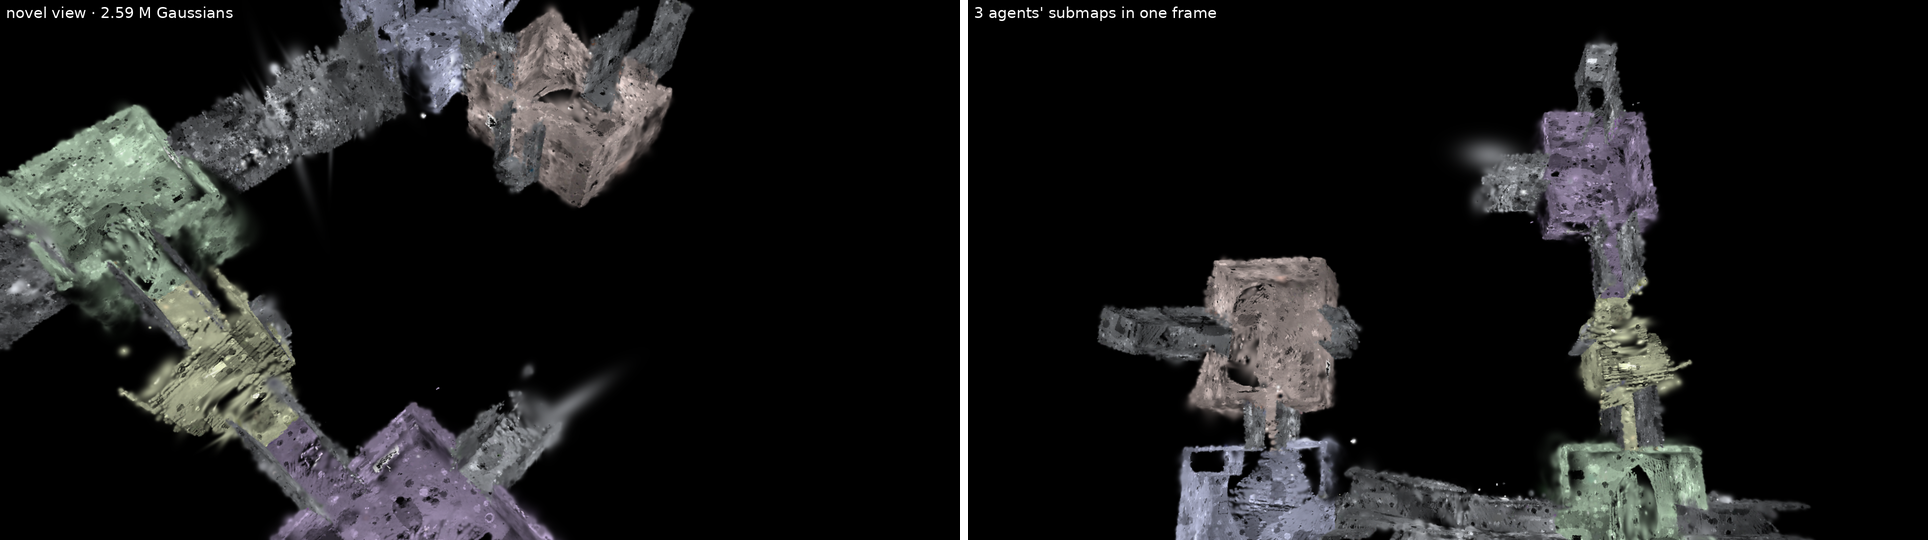
\includegraphics[width=\textwidth]{fig_splat.png}\\[0.4em]
  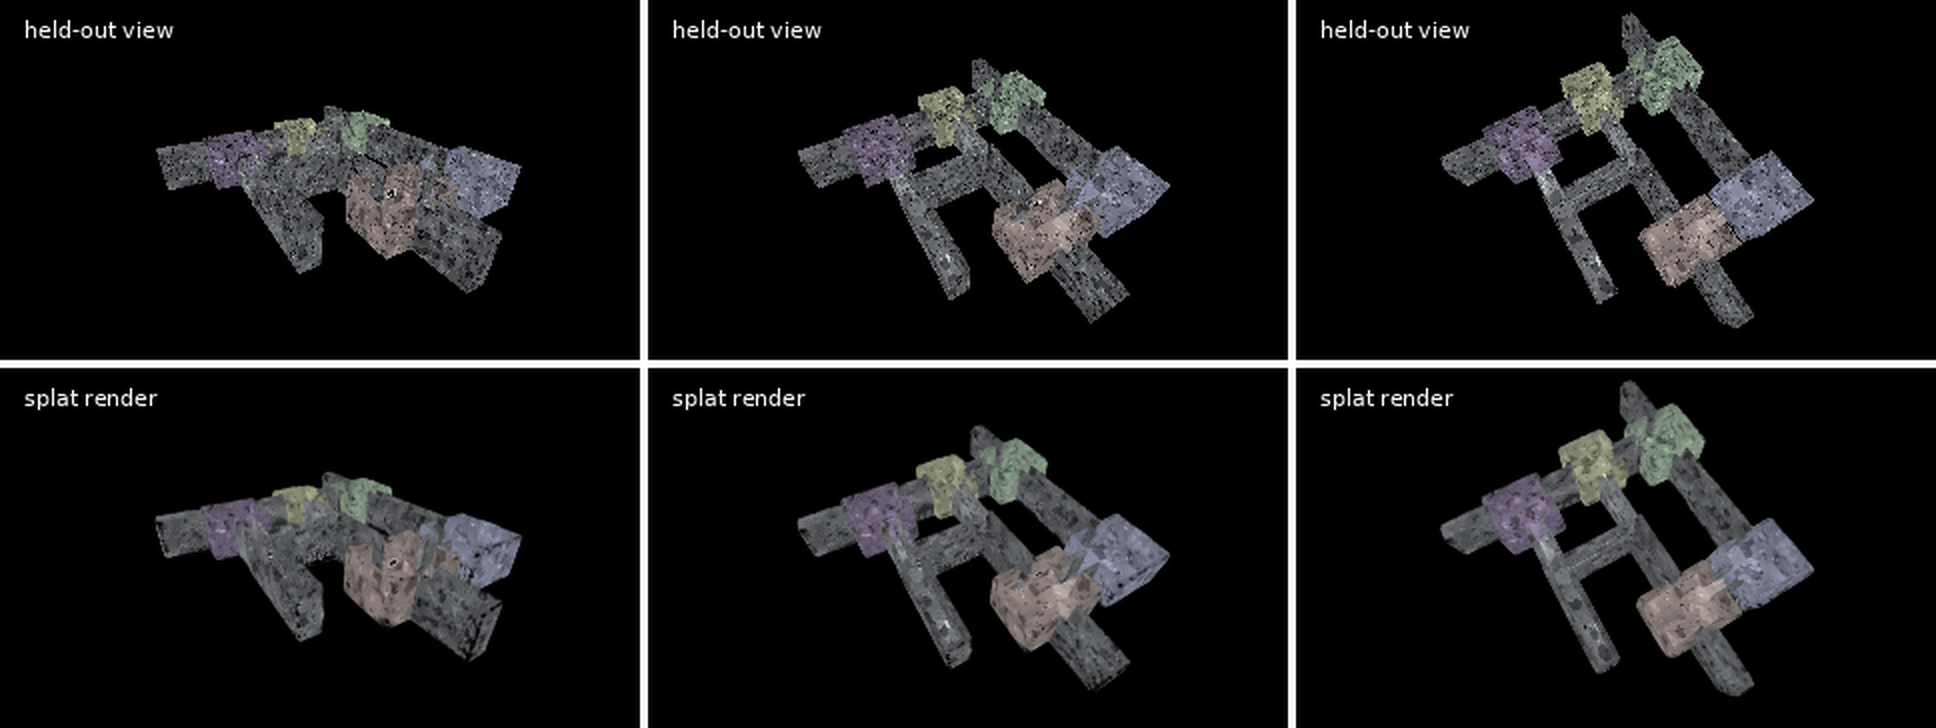
\includegraphics[width=0.75\textwidth]{fig_worldgen_heldout.png}
  \caption{Gaussian-splat reconstruction trained on AWS g4dn (T4). Top: a novel view and the per-agent submaps
  placed in one frame, from three agents' keyframes of a 200\,s mission (training \code{20261024T121121Z-gpu-ae604c},
  render \code{20261024T132853Z-gpu-1e9c60}; 2.59\,M Gaussians; training-view PSNR). Bottom: held-out views of the
  generated maze next to splat renders (run \code{20261026T211816Z-gpu-2705f3}, 3{,}000 steps, 187{,}405 Gaussians,
  held-out PSNR 24.36\,dB over 6 views, from 23.12\,dB at initialisation).}
  \label{fig:splat-renders}
\end{figure*}

\indentedheading{Implementation boundary and prior systems}

OpenCV 5 supplies the rectified imagery, stereo disparity, and
depth-uncertainty inputs. The reconstruction service implements
submap anchoring, depth seeding, lifecycle management, training
schedules, and atomic chunk publication. Differentiable
rasterization runs through gsplat/PyTorch; Spark/WebGL handles
interactive browser rendering.

Gaussian-SLAM informs the depth and loss recipe, RTG-SLAM
motivates stable/unstable Gaussian management, and LoopSplat
provides the closest precedent for rigid submap placement.
SplaTAM and Photo-SLAM demonstrate complementary approaches to
joint tracking and Gaussian mapping
\cite{gaussianslam,rtgslam,loopsplat,splatam,photoslam}.
Their published operating points use different sensors, scenes,
and hardware.

Ariadne's demonstrated reconstruction is an inspectable visual
layer over validated stereo-inertial geometry. The live service
connects three agents to a shared browser scene; the separate GPU
experiment establishes measurable refinement on synthetic data.
Together they define a functioning reconstruction interface and
its current quality and compute limits.




\section{OpenCV 5 in the working path}

Ariadne's path from camera observations to shared geometry passes repeatedly
through OpenCV 5. Image registration, sparse tracking, stereo reconstruction,
learned correspondence, robust geometric estimation, and nonlinear optimization
all execute through its C++ primitives. Ariadne supplies the stateful machinery
around them: landmark management, inertial factors, bundle adjustment, graph
consistency, communication policy, volumetric mapping, and mission planning.
This boundary makes it possible to examine both what OpenCV contributes and
whether the resulting system improves when a stronger primitive is introduced.

\indentedheading{Pinned implementation and numerical contracts}

The project builds OpenCV 5.0.0 and matching \code{opencv\_contrib} sources
from pinned commits, with C++17 and Eigen 3.4.1. The contrib build includes
\code{ximgproc}, \code{xphoto}, \code{optflow}, and \code{quality}; build-time
probes verify available headers, linked symbols, DNN engines, and stereo
interfaces~\cite{opencv5}. Run manifests record source revisions, the OpenCV
build-information identity, model hashes, thread settings, and configuration.
ROS 2 Jazzy and Gazebo Harmonic provide the simulated sensor environment,
while the geometry and replay libraries remain usable without ROS.

The pinned release exposed several consequential API details. It includes
\code{cv::ALIKED}, \code{cv::LightGlueMatcher}, and \code{cv::ANNIndex},
but has no native \code{cv::XFeat} class. OpenCV's learned-feature classes
also require externally supplied model weights. Its \code{cv::Volume}
interface supports volumetric fusion but does not expose the per-voxel
weight and read operations required by Ariadne's planner. These findings
were resolved against the installed implementation and retained as
explicit algorithm and dependency decisions.

\begin{table*}[t]
\centering
\small
\setlength{\tabcolsep}{5pt}
\renewcommand{\arraystretch}{1.13}
\begin{tabular}{@{}
    P{2.25cm}
    P{4.05cm}
    P{9.30cm}
@{}}
\toprule
\textbf{Stage} &
\textbf{OpenCV 5 primitives} &
\textbf{Implementation and measured evidence} \\
\midrule

Image preparation &
\code{imgproc}, \code{photo}, \code{xphoto};
rectification, remapping, filtering &
Stereo rectification, row correction, exposure normalization,
flat-field compensation, and optional variance-stabilized denoising.
Radiometric stages are separately gated and evaluated for their
effect on geometry. \\

Tracking and stereo &
\code{calcOpticalFlowPyrLK},
\code{buildOpticalFlowPyramid},
\code{StereoSGBM},
\code{DisparityWLSFilter} &
Pyramidal LK with forward/backward and epipolar rejection;
spatial ORB replenishment; metric disparity and uncertainty.
WLS confidence is implemented as an optional path, with unchanged
left disparity and an unmeasured confidence-quality AUC. \\

Learned perception &
\code{ORB}, \code{ALIKED},
\code{LightGlueMatcher},
\code{dnn::Net}, \code{ANNIndex} &
Ariadne-assembled XFeat graph, EigenPlaces retrieval,
and native ALIKED--LightGlue verification. Reference-output
agreement is tested; exact cosine search is the retrieval default.
Learned keyframe matching reaches $0.607$ pose AUC at $10^\circ$. \\

Geometric verification &
\code{findFundamentalMat},
\code{findEssentialMat},
\code{solvePnPRansac},
\code{triangulatePoints} &
Seeded USAC, reprojection checks, stereo relative-pose
estimation, and covariance-aware degeneracy rejection.
Verified constraints subsequently enter Ariadne's PCM
and robust graph backend. \\

State estimation &
\code{detail::LevMarqBase},
\code{solvePnPRefineLM},
\code{projectPoints} &
OpenCV drives nonlinear iterations; Ariadne assembles
visual-inertial residuals, analytic SE(3) Jacobians,
Schur elimination, covariance, and sparse graph systems.
Numerical checks agree with independent PnP and GTSAM oracles. \\

Volumetric planning &
\code{ptcloud}, \code{PCA},
\code{filter2D}, \code{parallel\_for\_} &
OpenCV supplies a fusion oracle, frontier-clustering and
support primitives, and parallel scoring. Ariadne implements
the production voxel-hash TSDF, incremental 3D ESDF,
responder clearance, and route search. \\

Visualization and routing &
\code{findContours},
\code{approxPolyDP};
image and depth utilities &
Contour geometry supports the experimental visibility graph;
validated stereo depths initialize Gaussian submaps.
The Gaussian trainer, browser renderer, and D* Lite egress
solver are separate implementations. \\

\bottomrule
\end{tabular}
\caption{OpenCV 5 interfaces exercised by Ariadne and the corresponding
system-level implementations. Numerical agreements, subsystem gains,
and optional paths are distinguished by their reported evaluation
conditions.}
\label{tab:opencv5-working-path}
\end{table*}

\indentedheading{Visual primitives and learned inference}

At frame rate, \code{cv::calcOpticalFlowPyrLK} propagates existing tracks
through a three-level pyramid with a $21$-pixel window. Forward/backward
checks and seeded USAC fundamental-matrix estimation remove inconsistent
motion. ORB replenishes features on an $8\times6$ grid, maintaining a
target of $400$ active tracks. When landmark-bearing tracks fall below
$30$, descriptor re-association against healthy local landmarks is
followed by seeded PnP, requiring at least $12$ inliers before track
identities are restored. Stereo depth comes from rectified
\code{StereoSGBM}, with disparity uncertainty propagated into landmark
admission and subsequent optimization.

Stereo implementation details affected accuracy directly. Online
right-image row refinement reduced the median vertical residual on
EuRoC V2\_01 from $1.46$ to $0.09$ pixels. Left/right exposure matching
improved correspondence stability under unequal camera response.
An optional \code{ximgproc::DisparityWLSFilter} path computes confidence
using right disparity and weighted filtering; preserving the original
left matcher avoids a factory-side parameter mutation observed in the
pinned API. At $752\times480$, this path adds approximately $37$\,ms
per stereo pass. It remains off by default because its confidence
discrimination has not been measured against the planned reference.
The release also treats nonpositive \code{disp12MaxDiff} as a strict
consistency setting, which required explicit parameter validation.

The learned front end illustrates how API-level implementation and
trajectory evaluation informed one another. Ariadne assembled XFeat's
forward graph directly through \code{cv::dnn::Net::addLayer} and
\code{connect}, using OpenCV convolution, activation, pooling, resize,
and elementwise operations. Batch normalization is folded into
convolution weights, while the $8\times8$ spatial unfold is expressed
as a fixed stride-eight convolution. An independent
\code{cv::gemm}-based engine provides an operation-level reference.
The runtime graph reproduces upstream feature maps within
$8\times10^{-6}$ relative error, all $4096$ tested keypoint positions,
and descriptor cosine agreement of $1.000000$. Both engines use
credited upstream weights; model training was outside Ariadne's scope.

That numerical fidelity did not translate into better local odometry.
XFeat reduced lost tracks but increased EuRoC trajectory error on six
of seven previously passing flights. Keyframe cadence and matcher
variants failed to reverse the pattern, so ORB remains the adopted
EuRoC VO feature path. Learned inference instead serves recognition
events where stronger appearance matching can change the graph
\cite{orb,xfeat}.

EigenPlaces R50-256 runs through \code{cv::dnn} with one network
instance per thread. Its $256$-dimensional descriptors are compared
by exact cosine search using an OpenCV matrix product.
\code{cv::ANNIndex} remains a scale and persistence ablation:
on $297$ EuRoC revisit queries, approximate and exact indices
returned identical top-ranked results. EigenPlaces achieved
\textbf{$0.626$ R@1} at $376\times240$, against $0.444$ for
mean-bit retrieval and $0.167$ for random selection; the larger
$752\times480$ model reached $0.677$. The smaller export was
retained for its substantially lower inference cost.
The evaluated simulator revisits reached $0.705$ R@1 at
$640\times360$~\cite{eigenplaces}.

Selected overlaps proceed to \code{cv::ALIKED} and
\code{cv::LightGlueMatcher}. Ariadne exported ALIKED-n16 and the
nine-layer LightGlue model from pinned upstream weights, adapting
the ONNX graphs for OpenCV's DNN engine. The export preserves
upstream coordinate normalization by passing pre-normalized
keypoints through \code{setPairInfo}; using OpenCV's per-axis
normalization would change the model's intended coordinate frame.
Reference tests report keypoint differences below
$9.3\times10^{-5}$ pixels, descriptor differences below
$4\times10^{-6}$, and identical match sets.

On $4{,}815$ EuRoC retrieval candidates across $11$ flights,
ALIKED--LightGlue raised pose AUC at $10^\circ$ from
\textbf{$0.284$ to $0.607$} against ORB, improving or matching
every flight. Geometric average precision over the fixed
$676$ positive pairs rose from $0.303$ to $0.807$, and
LightGlue contributed another $0.042$ AUC over ALIKED with
mutual-nearest-neighbour matching. Increasing the keypoint cap
from $1024$ to $2048$ brought no measured pose improvement
at approximately $2.8\times$ the compute cost
\cite{aliked,lightglue}.

Four confident false verifications nevertheless retained
$210$--$264$ essential-matrix inliers despite rotation errors of
$37^\circ$--$59^\circ$. Ariadne consequently keeps stereo PnP,
covariance and degeneracy checks, pairwise consistency, and robust
graph optimization after learned matching. The front-end score
measures correspondence quality; the shared map changes only
after the full geometric acceptance path succeeds.

\indentedheading{OpenCV optimization and Ariadne's estimator}

The stereo-inertial estimator uses OpenCV's
\code{cv::detail::LevMarqBase} as its nonlinear iteration driver.
Ariadne implements the backend: manifold residuals, exact
left-perturbation SE(3) Jacobians, landmark Schur elimination,
sparse normal-equation assembly, gauge fixing, and covariance
recovery. OpenCV's driver controls damping and step acceptance;
the reduced systems are factored with Eigen. For the windowed
visual-inertial problem, the damped normal equations have the
block structure

\begin{equation}
\begin{bmatrix}
H_{ss}+D_s & H_{sl}\\
H_{ls} & H_{ll}+D_l
\end{bmatrix}
\begin{bmatrix}
\delta s\\
\delta l
\end{bmatrix}
=
-
\begin{bmatrix}
g_s\\
g_l
\end{bmatrix},
\qquad
H_{\mathrm{red}}
=
H_{ss}+D_s-
H_{sl}(H_{ll}+D_l)^{-1}H_{ls},
\label{eq:opencv-schur}
\end{equation}

where $s$ contains pose and inertial states and $l$ contains
landmarks. Independent landmark blocks are eliminated before
solving the reduced state system. The adopted window contains ten
keyframes and includes stereo reprojection, preintegrated IMU,
and bias random-walk factors.

The split is checked numerically. The pose-graph solver agreed
with GTSAM 4.3 on \textbf{$100/100$} seeded synthetic graphs,
with worst relative energy difference
$1.5\times10^{-12}$. A one-free-pose bundle-adjustment problem
agreed with \code{cv::solvePnPRefineLM} within
$1.3\times10^{-9}$\,m and $2.8\times10^{-9}$\,rad;
analytic Jacobians, Schur solutions, and selected covariance
blocks also passed independent checks. The built-in
\code{cv::detail::PoseGraph} optimizer was unsuitable for the
pinned configuration, which lacked its required Eigen-enabled
build path. Ariadne therefore retains its own SE(3) graph
representation and optimizer behind the OpenCV LM interface.

On all $11$ EuRoC flights, the complete stereo-inertial
estimator achieved mean RMS ATE of $0.120$\,m, improving
to \textbf{$0.066$\,m} with loop closure. The latter fell
within the stated published stereo-inertial comparison class
on $10/11$ flights and matched or improved the published
ORB-SLAM3 result on $7/11$. These are comparisons with
published references under the report's stated alignment
protocol; V1\_03 remains the principal outlier at $0.288$\,m.

\indentedheading{Beyond the camera front end}

OpenCV's geometry and image interfaces continue into planning
without carrying its system state. The evaluated
\code{cv::Volume} implementation serves as a fusion comparison;
Ariadne's production mapper maintains $5$\,cm voxel-hash TSDF
blocks with explicit observation weights, tri-state occupancy,
and incremental 3D ESDF queries. \code{cv::PCA} assists frontier
partitioning, \code{cv::filter2D} aggregates local support and
risk statistics, and \code{cv::parallel_for\_} distributes
independent view scoring. Contour extraction and polygonal
approximation support the experimental FAR-style visibility
graph. D* Lite, CBBA, geometric risk estimation, and Gaussian
submap management are implemented separately.

Camera-model support also mattered outside EuRoC.
The Hilti 2023 evaluation introduced equidistant
Kannala--Brandt cameras through
\code{cv::fisheye::stereoRectify},
\code{cv::fisheye::initUndistortRectifyMap}, and
\code{cv::fisheye::undistortPoints}.
Synthetic calibration checks reached $10^{-3}$-pixel
row agreement and relative depth error below $10^{-4}$.
The real low-light transfer result remained negative,
with $0/100$ on all three evaluated Hilti configurations.
Correct camera-model handling therefore established a valid
measurement pipeline without rescuing the estimator's
out-of-domain performance.

\indentedheading{Compute profile and reproducibility}

Measured inference costs explain the runtime division.
On a four-thread \code{g4dn.xlarge} CPU, median inference
was $311.8$\,ms for EigenPlaces at $640\times360$,
$1998.6$\,ms for ALIKED at $1280\times720$, and
$921.0$\,ms for a warm LightGlue pair. Two ALIKED
extractions and one LightGlue match cost roughly five
seconds on that CPU configuration. Continuous LK tracking
and event-driven learned matching follow directly from
these measurements.

Optimization experiments were held to the same numerical
and behavioral criteria as the mapping experiments.
A proposed ALIKED graph rewrite reduced eight-thread
median inference from $1112.7$ to $469.9$\,ms but changed
one verification verdict and exceeded the preregistered
descriptor tolerance; it was rejected. Reducing the
keypoint cap to $512$ lost four accepted pairs, while
alternative descriptor wire codings failed their adoption
criteria despite substantial byte savings. These results
kept the accepted matching configuration stable through
the measured communication experiments.

The estimator produced bit-identical trajectories with
OpenCV thread pools of $2$, $5$, and $16$ on the tested
three-agent replay. Other OpenCV DNN paths, particularly
ALIKED, showed thread-dependent output differences and
retain an explicit per-thread execution contract.
Performance profiling located a substantial live bottleneck
in per-agent image ingestion and lens processing. Disabling
the unnecessary lens path improved the tested runtime;
a subsequent pipelined-ingestion variant changed real-time
factor from $0.839$ to $0.833$, within noise, and remains
disabled by default.

A native OpenCV 5.0.0 and contrib build also passed its
Arm smoke checks on AWS Graviton4, the COOL stack.
In selected 16-thread
measurements, ALIKED at $1280\times720$ required
$530$\,ms on c8g against $829$\,ms on c7i,
a runtime ratio of $0.64$; LightGlue and EigenPlaces
reached ratios of approximately $0.85$--$0.88$.
These compare stock OpenCV builds on different processors.

The final recorded AWS pre-merge gate passed $54/54$
integration checks and $708/708$ C++ tests using the
pinned OpenCV environment. Its render was reused, and
the scientific results above retain their individual
dataset, seed, revision, and run-manifest provenance.
Reproducibility is strongest at these recorded boundaries:
MCAP replay, seeded geometric estimation, reference-model
agreement, and explicitly versioned build artifacts.
Floating-point execution and SIMD selection still require
architecture-specific checks.

Across these experiments, OpenCV 5 provides a substantial
and testable computational foundation. Its primitives
support both classical geometry and learned perception,
while measured accuracy, numerical agreement, communication
cost, and execution time determine which configurations
enter Ariadne's working path.




\section{What the experiments establish}

Ariadne's experiments follow the path of information through the system:
from a visual correspondence to an estimated pose, from local trajectories
to a consistent shared map, and from observed geometry to an actionable
route. Each stage was evaluated against a matched baseline, an independent
numerical oracle, or ground truth. Together, these measurements explain
the architecture that emerged from implementation, including several
choices that changed when their expected benefits failed to materialize.

\begin{table*}[t]
\centering
\footnotesize
\setlength{\tabcolsep}{4pt}
\renewcommand{\arraystretch}{1.15}
\begin{tabular}{@{}P{2.4cm}P{9.65cm}P{3.75cm}@{}}
\toprule
\textbf{Subsystem} & \textbf{Measured result} & \textbf{Evaluation} \\
\midrule

Local matching &
ALIKED--LightGlue raised pose AUC@$10^\circ$ from
\textbf{0.284 to 0.607}; geometric AP rose from 0.303 to 0.807.
&
4,815 matched EuRoC pairs, 11 flights; ORB baseline.
\\

Place recognition &
EigenPlaces reached \textbf{0.626 R@1}, against 0.444 for mean-bit
and 0.167 for random retrieval. Int8 descriptors preserved
top-1 results at 258 B versus 1,024 B.
&
297 EuRoC queries; exact and approximate index agreement.
\\

Stereo-inertial SLAM &
Loop closure reduced mean ATE from \textbf{0.120 to 0.066 m};
the final trajectory matched or improved published ORB-SLAM3
results on 7/11 flights.
&
Same-run EuRoC ablation; published-system reference.
\\

Numerical estimation &
Pose-graph optimization agreed with GTSAM on
\textbf{100/100} graphs, with relative energy error
$\leq1.5\times10^{-12}$; seven SE-Sync benchmark
graphs received valid certificates.
&
Independent numerical and optimization oracles.
\\

Robust collaboration &
Known-entry gating reduced worst scene-0 seed-mean
merged ATE from 3.79 m to \textbf{0.014675 m},
retaining all \textbf{560} tested true edges.
&
Paired gated/ungated multi-agent experiments.
\\

Budgeted exchange &
Spectral selection reached \textbf{0.970} mean
utility relative to exact optimum, against 0.936
for greedy selection.
&
60 enumerated synthetic instances.
\\

Volumetric mapping &
TSDF coverage improved from 0.933 to
\textbf{0.942}; occupied precision rose from
0.707 to \textbf{0.865}.
&
Matched replay against the initial occupancy mapper.
\\

Traversability and risk &
Responder traversability achieved
\textbf{1.000 precision, 0.900 recall};
the structural-risk proxy reached AUC 0.831.
&
Ground-truth traversability and procedural hazard labels.
\\

Safe egress &
All \textbf{12/12} planned routes were ground-truth valid;
the final 4.44142 m route matched the reference geodesic.
D* Lite used 7.6$\times$ fewer vertex expansions.
&
Mission spool and 180 randomized graph updates.
\\

Exploration and allocation &
CBBA matched centralized greedy on
\textbf{40/40} replans, averaging 0.994 of the
exact optimum in linked cases. Ariadne attained
0.757 final maze coverage.
&
Two-agent allocation replay; six-policy exploration sweep.
\\

Active exposure &
Recovered from a two-stop overexposure in
\textbf{2.35 s}, reducing ATE from 19.1 to
16.1 mm against fixed exposure.
&
Matched degraded-vision replay.
\\

Gaussian reconstruction &
Synthetic training-view PSNR improved from
\textbf{22.2 to 25.1 dB}; the live three-agent
service produced 259,994 Gaussians across four submaps.
&
T4 training experiment; 20 s live reconstruction.
\\

Agentic orchestration &
Bedrock completed 100 joint replans over
500 simulated seconds; classical and model-driven
runs each reproduced their recorded state in two replays.
&
Matched two-agent live chooser experiment.
\\

System validation &
Estimator trajectories were bit-identical across
2, 5, and 16 OpenCV threads; the AWS integration
gate passed \textbf{54/54} checks and
\textbf{708/708} C++ tests.
&
Seeded MCAP replay and pinned AWS build.
\\

\bottomrule
\end{tabular}
\caption{Principal experimental results, retaining the comparator and
evaluation setting for each claim. Matched ablations, numerical oracles,
and published-system references are identified separately.}
\label{tab:wins}
\end{table*}

\indentedheading{What the comparisons reveal}

The strongest trajectory result is the effect of loop closure on
the same eleven EuRoC flights, reducing mean error by approximately
45\%. The final 0.066 m mean compares with ORB-SLAM3's published
0.035 m mean, while improving or matching its reported result on
seven individual sequences~\cite{orbslam3}. The numerical backend
was independently checked against GTSAM, OpenCV PnP refinement,
and SE-Sync objectives~\cite{sesync}; its agreement confirms the
estimation machinery underlying the dataset experiments.

Collaboration produced the largest change in map reliability.
A known-entry Mahalanobis gate, followed by PCM and GNC-TLS,
suppressed metre-scale false merges to centimetre-scale error.
In synthetic outlier campaigns, PCM--GNC handled up to 90\%
false closures in groups of ten and 70\% in two growing
clusters, while retaining planted true connections. Spectral
exchange achieved near-optimal connectivity utility on the
evaluated small instances, supporting the communication-aware
selection developed from Tian et al.\ and the sparse
collaboration principles of Swarm-SLAM and Kimera-Multi
\cite{tian2018near,lajoie2024swarmslam,tian2022kimeramulti}.

The geometric map carried these estimates into responder-scale
decisions. Five-centimetre TSDF fusion improved occupied-space
precision, hybrid body clearance preserved traversable passages,
and all twelve evaluated egress routes agreed with ground-truth
passability. Incremental D* Lite reproduced exact shortest-path
solutions after randomized map changes~\cite{dstar2002}.
The corresponding multi-agent allocator reached 99.4\% of
the exact assignment score on its evaluated linked replans,
with sparse consensus traffic of 11.8 kB against 123.4 kB
for dense exchange~\cite{cbba}.

The implementation also closes the operational loop. Live
sensing, planning, movement, multi-agent communication, model
orchestration, and the browser console share recorded mission
state. Gaussian submaps turn the resulting observations into
an inspectable scene, while deterministic replay preserves
the geometric and decision traces. The reconstruction trainer's
synthetic quality measurements and the live multi-agent streaming
results characterize their respective compute paths.

\indentedheading{Decisions shaped by experiments}

Several promising designs were revised after direct evaluation.
XFeat reproduced its upstream network accurately and reduced
tracking losses, but increased trajectory error on six of seven
passing EuRoC flights; ORB remained the local VO feature.
An ALIKED graph optimization achieved 2.37$\times$ faster
inference but changed geometric-verification decisions, so
the verified graph was retained. Lower-bit local descriptors
likewise remained experimental after failing the registered
adoption criteria.

The next-best-view planner improved coverage per metre and
eventual map completion, reaching 0.757 coverage on the maze
against 0.713 for coverage-greedy. Its preregistered
coverage-time AUC nevertheless ranked third of six policies
in both scenes. Execution traces identified repeated turning
as the principal cost, motivating heading-aware command
planning. A concurrent ingestion optimization intended to
raise real-time factor from approximately 0.84 toward 1.0
instead measured 0.833 against 0.839 for its control and
was discarded.

Degraded-vision experiments further clarified the operating
regime. Active exposure recovered from saturation, while
brightness-matched carried illumination remained harder for
geometric tracking than fixed lighting. Transfer to the
Hilti 2023 low-light sequences failed the established accuracy
criterion across all three configurations, and realistic,
temporally correlated dust modelling remained outside the
completed evaluation. These findings delimit the tested
visual conditions and preserve concrete directions for
subsequent robustness work.

The resulting system combines classical geometric estimation,
selective learned perception, robust multi-agent consensus,
volumetric planning, and task-level orchestration. Its principal
contribution lies in how these components exchange evidence:
candidate observations are priced before transmission, geometric
constraints are checked before merging, and responder routes
are grounded in observed clearance. The experiments demonstrate
that this discipline can preserve map consistency and produce
usable routes even when individual visual matches and
communication opportunities are unreliable.



\section{AWS deployment, accelerated vision, and reproducibility}

Ariadne's operator console frontend is hosted on AWS at
\url{https://www.ariadne.cynicpixel.xyz/} (Cloudflare DNS, Amazon CloudFront,
S3 origin). The hosted page serves the console with a generated scene; the
live simulation worker is not attached to it, and a live run is
demonstrated by screen share on request. The deployment brings together OpenCV-based estimation,
collaborative mapping, Amazon Bedrock task decisions, and Gaussian
reconstruction. The same software can consume live simulator streams
or recorded MCAP observations, allowing an operator-visible mission
to be examined again under identical inputs.

\indentedheading{Cloud architecture and operator interface}

The deployment separates CPU geometry, GPU rendering, model
orchestration, and persistent artifacts. EC2 c7i instances provide
high-throughput replay and evaluation; Graviton4 c8g/m8g instances
host the arm64 OpenCV execution path; GPU instances support Gazebo
and Gaussian reconstruction. Amazon Bedrock Converse invokes Nova
2 Lite for bounded task-level decisions, while S3 and ECR preserve
recordings, results, and container images.

\begin{figure*}[t]
\centering
\resizebox{0.96\linewidth}{!}{%
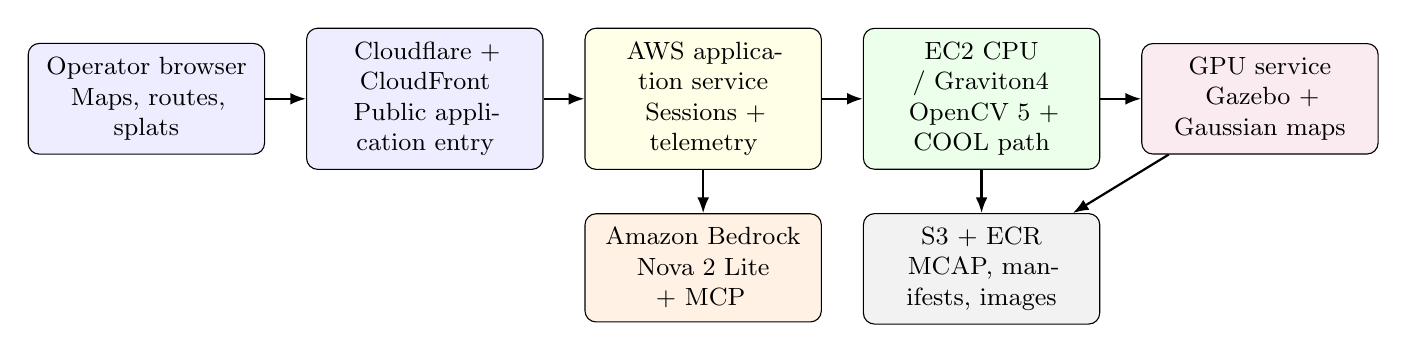
\begin{tikzpicture}[
    node distance=0.45cm and 0.52cm,
    >=Latex,
    box/.style={
        draw,rounded corners,align=center,
        text width=2.65cm,minimum height=0.90cm,
        font=\small,inner sep=5pt
    },
    link/.style={-{Latex[length=2mm]},thick}
]
\node[box,fill=blue!7] (ui)
    {Operator browser\\Maps, routes, splats};

\node[box,fill=blue!7,right=of ui] (edge)
    {Cloudflare + CloudFront\\Public application entry};

\node[box,fill=yellow!10,right=of edge] (app)
    {AWS application service\\Sessions + telemetry};

\node[box,fill=green!8,right=of app] (cpu)
    {EC2 CPU / Graviton4\\OpenCV 5 + COOL path};

\node[box,fill=purple!8,right=of cpu] (gpu)
    {GPU service\\Gazebo + Gaussian maps};

\node[box,fill=orange!10,below=0.55cm of app] (llm)
    {Amazon Bedrock\\Nova 2 Lite + MCP};

\node[box,fill=gray!10,below=0.55cm of cpu] (store)
    {S3 + ECR\\MCAP, manifests, images};

\draw[link] (ui)--(edge);
\draw[link] (edge)--(app);
\draw[link] (app)--(cpu);
\draw[link] (cpu)--(gpu);
\draw[link] (app)--(llm);
\draw[link] (cpu)--(store);
\draw[link] (gpu)--(store);
\end{tikzpicture}%
}
\caption{Ariadne's AWS deployment architecture. The browser exposes
mission telemetry and reconstruction, CPU services maintain geometry,
GPU services process simulation and Gaussian maps, and Bedrock
handles bounded task-level decisions. Versioned artifacts connect
live execution with reproducible evaluation.}
\label{fig:aws-deployment}
\end{figure*}

The FastAPI operator service exposes session controls, recorded
playback, and WebSocket telemetry. Its interface shows agent
trajectories, camera feeds, tracked features, communication traffic,
map uncertainty, exploration tasks, and responder routes. The
three-agent console records camera feature overlays with 491,
371, and 298 points in one demonstrated frame; the collaboration
panel exposes verified inter-agent edges and measured bytes,
with controls for link interruption, restoration, and false-edge
injection. A separate reconstruction pane renders Gaussian submaps
through Spark 2.3.1 and Three.js 0.180.0, alongside a distinctly
labelled ground-truth scene.

\indentedheading{OpenCV 5, COOL, and native Graviton execution}

The CPU vision pipeline was structured around OpenCV operations
that recur across every agent and frame: rectification and
\code{cv::remap}, image conversion, pyramidal LK, filtering,
stereo preparation, resizing, and feature preprocessing.
These stable interfaces also define the Graviton acceleration
workload, independently of which optional restoration or learned
feature variants survive evaluation.

Ariadne pins OpenCV and \code{opencv\_contrib} to 5.0.0.
The corresponding Graviton4 COOL distribution is OpenCV's
Cloud Optimized OpenCV 3.1, built on the OpenCV 5.0 line
with Arm-specific optimizations. Its published C++ SDK resides
under \code{/opt/cool/cpp\_sdk}; the build configuration can
select its CMake package through
\code{OpenCV\_DIR=/opt/cool/cpp\_sdk/lib/cmake/opencv4}.
The vendor's CMake directory retains the historical
\code{opencv4} name despite the OpenCV 5 implementation.
The same source tree also builds against the project's
stock arm64 OpenCV installation.

Reproduction is defined at the library boundary.
\code{infra/docker/core.Dockerfile},
\code{docker-bake.hcl}, \code{infra/scripts/core.sh},
and the root CMake configuration establish the pinned
build. The COOL preparation path is documented by
\code{infra/cool/day1.sh}, \code{infra/cool/probe.cpp},
and the \code{spinup.sh} COOL profile. The build uses
\code{CMAKE\_SKIP\_RPATH=ON} and checks installed binaries
for embedded RPATH/RUNPATH, preserving selection through
\code{LD\_LIBRARY\_PATH}. Each run records the active
OpenCV version, CPU features, and an FNV-1a hash of
\code{cv::getBuildInformation()} obtained from the loaded
library. This identifies the actual binary implementation
used to process a recording.

The native Graviton4 baseline was exercised on c8g with
OpenCV 5.0.0 and contrib. At 16 threads, ALIKED inference
at $1280\times720$ measured \textbf{$530$\,ms} on c8g
against $829$\,ms on c7i, or $0.64\times$ the x86
execution time. LightGlue and EigenPlaces measured
approximately $0.85$--$0.88\times$ the corresponding
x86 times. These stock-build comparisons establish the
arm64 workload baseline; a COOL measurement is produced
by the \code{infra/cool/day1.sh} protocol and identified by
its loaded-library manifest.
The controlled COOL comparison uses identical inputs,
instance type, thread settings, and executable, with
the OpenCV implementation as the experimental variable.

\indentedheading{Seeded simulation and recorded missions}

The evaluation environment is generated on a $6$\,m
room-maze lattice, with seeded corridors, loops, dead ends,
entrances, target regions, and responder-scale bottlenecks.
Scene identity records the generator version, preset digest,
seed, and accepted generation attempt. Gazebo Harmonic renders
stereo imagery under configurable illumination, while ROS 2
Jazzy connects cameras, IMU streams, movement, and operator
interfaces. Collision-checked kinematic motion provides
canonical poses and inertial references.

Sensor streams, motion, calibration, and ground truth are
recorded into MCAP. Replay applies seeded image degradation
and IMU perturbations to the same observations, permitting
matched algorithm comparisons without repeated scene rendering.
Run manifests identify source revisions, image digests,
OpenCV build fingerprints, model weights, agent count,
thread settings, seeds, and planner configuration.

The three-agent, $200$-second mission supplied a particularly
useful systems stress test. Its recording contains $4{,}001$
estimator poses per agent. A synchronization defect exposed
by replay disagreement was corrected, after which two
replays reproduced the recorded trajectory state exactly.
On c7i.4xlarge, trajectories also remained bit-identical
with OpenCV thread pools of $2$, $5$, and $16$.
Subsequent profiling located the principal CPU cost in
per-agent frame ingestion, guiding the adopted thread-pool
and lens-processing configuration.

\indentedheading{Bedrock orchestration and live interaction}

The live planner submits a joint decision context to Nova
2 Lite through Bedrock Converse. MCP tools expose map
renderings, uncertainty, routes, candidate tasks, and agent
state. Model responses select planner-generated candidates
and supply rationales; the deterministic runtime validates
the selections and dispatches commands. The console presents
these decisions alongside the observations and route state
that informed them.

The first accepted $90$-second experiment completed
$18$ joint replans and $36$ per-agent model assignments
without a provider error or fallback. A matched
classical--Bedrock experiment subsequently held the scene,
seed, renderer, runtime, and source revision fixed.
Bedrock changed agent 0's selection on $6/18$ replans
and chose the highest-ranked candidate $31/36$ times,
against $26/36$ for the classical chooser. Both arms
passed deterministic replay checks.

The longer matched experiment ran for $500$ simulated
seconds. Each chooser completed \textbf{$100$ joint
replans and $200$ commands}, recording $10{,}001$
frames per agent. Two independent replays per arm
reproduced the live state digests and each other exactly.
The $90$-second Bedrock arm measured $5.8$\,s median
and $7.45$\,s p90 orchestration latency, including
tool interactions. These experiments establish sustained
multimodal tool orchestration, controlled behavioral
differences, and a reproducible decision trace.

\indentedheading{GPU reconstruction and artifact delivery}

The GPU reconstruction service receives rectified RGB,
stereo depth, uncertainty, and anchor-relative poses
through a bounded keyframe stream. Its gsplat/PyTorch
path supports incremental Gaussian refinement and
exports atomic \code{.splat} chunks with independently
versioned placement transforms. The browser renders
these chunks using client-side WebGL, allowing incident
command to inspect the reconstructed interior from
new viewpoints.

In the three-agent integration, $71$ keyframes arrived
without transport drops and produced four submaps,
\textbf{$259{,}994$ Gaussians}, and $8.3$\,MB of
browser-ready geometry. A separate Tesla T4 training
experiment improved median synthetic training-view
PSNR from $22.2$ to $25.1$\,dB over $60$ keyframes.
The live streaming and GPU-training results retain
distinct run identifiers, while sharing the same
submap and export contracts.

Terraform manages networking, IAM, compute, ECR,
versioned S3 storage, and budget controls. Containers
and artifacts are published with digests; private
buckets use encryption, TLS-only access, and lifecycle
policies. GitHub OIDC supplies scoped CI credentials,
while EC2 jobs use IMDSv2, SSM, and automatic termination.
A host-side Spot dispatcher schedules CPU evaluation jobs.

The recorded AWS pre-merge gate passed
\textbf{$54/54$ checks and $708/708$ C++ tests}
in $999$\,s, at approximately US\$0.035 of Spot
compute. The measured three-agent replay reached
real-time factor $0.836$ on c7i.4xlarge. Together,
the cloud execution, public entry point, operator
interface, model traces, and versioned artifacts
provide a reproducible route from simulated observation
to collaborative map, selected action, and visual
inspection.

\section{Limitations and operating envelope}

Ariadne's strongest evidence comes from reproducible stereo-inertial
estimation, robust map merging, volumetric planning, and multi-agent
mission execution. These capabilities have been evaluated through
public datasets, seeded simulation, numerical oracles, and recorded
cloud runs. Their operating envelope remains shaped by the geometry
and sensing assumptions of those experiments.

Perceptual aliasing remains a central challenge when agents have
unknown relative starting poses. Known-entry constraints substantially
improve map-merging reliability, while PCM can still admit a mutually
consistent cluster of false closures. Real-world visual transfer is
also demanding: the Hilti low-light evaluation exposed tracking
failures during difficult turning sequences, and the adopted
next-best-view policy did not meet its coverage-versus-time objective.
These results motivate stronger geometric disambiguation and
motion-aware exploration.

The simulator captures occlusion, illumination, sensor degradation,
and responder-scale obstruction, while leaving particulate dust,
material fracture, and evolving structural collapse outside its
physical model. Structural risk is consequently a geometric
planning proxy. Responder routes are validated against observed
clearance in the evaluated environments; field operation would
require physical-robot testing, additional environmental sensing,
and independent safety validation. These boundaries define the
next experimental questions for Ariadne's mapping and
decision-support architecture.

\section{Responsible use and human authority}

Ariadne is intended to support trained responders and incident
commanders by presenting observed geometry, traversability,
uncertainty, structural-risk indicators, and alternative egress
routes. These outputs inform human judgment; a planning score
does not authorize entry into a hazardous space. The system
requires no personal identification or persistent identity
tracking. Its representation concerns the environment:
surfaces, observations, agent state, and routes.

Human authority is preserved through explicit approval policies
and deterministic planning boundaries. The risk-gate and approval
workflow are implemented, although the evaluated live Bedrock
missions did not trigger an operator intervention; rejection
and fallback dispatch still require end-to-end validation.
Unknown space remains excluded from responder traversability,
and structural-risk scores remain geometric proxies.
Operational rescue use would require physical validation,
professional structural assessment, and accountable human
command. Ariadne is deployed as a research decision-support
system within these boundaries.


\section{Reproducibility and evidence trail}

Ariadne's repository is both the implementation and the experimental
record. Each result is tied to its inputs, executable, configuration,
and evaluation procedure, allowing the path from recorded observation
to reported measurement to be reconstructed. The central mechanism is
record-once simulation: Gazebo renders a mission into MCAP, while
estimation, collaboration, planning, and ablation experiments consume
the same observations through a ROS-independent replay interface.
This separates algorithmic differences from changes in rendering,
sensor timing, or simulated motion.

\indentedheading{Deterministic input and replay contract}

A procedural scene is identified by its generator revision, preset
digest, seed, and accepted generation attempt. Its geometry, routes,
and kinematic trajectories follow from those inputs. ROS 2 Jazzy and
Gazebo Harmonic produce rendered stereo observations; analytically
sampled ground-truth poses and IMU measurements are written into a
separate canonical MCAP stream. The two streams are merged by message
header timestamp, with topic name breaking ties. Camera observations
come from \code{sensors/}, while inertial and reference poses come
from \code{canonical/}.

This separation addresses a measured recording failure: the live
transport lost an IMU sample in a 199-second mission despite
delivering the remaining analytic values correctly. Canonical
streams instead use the same trajectory sampler as the kinematic
mover, with exact sampling grids and zero-initialized CDR padding.
The recorder verifies expected topics, stereo pairing, message
counts, timestamp intervals, and agreement with an independent
trajectory evaluator before accepting a mission. Canonical content
is additionally hashed over ordered
$(\mathrm{topic},\mathrm{timestamp},\mathrm{payload})$ tuples,
independently of MCAP container compression.

Two complementary MCAP interfaces preserve the execution path.
The ROS-compatible reader decodes recorded Image, CameraInfo, IMU,
PoseStamped, TF, and Clock messages directly through bounded XCDR1
parsers. Internal replay files retain Ariadne's framed wire messages,
including their production serialization headers, so replay
exercises the same decoding and byte-accounting routines as
communication between agents. MCAP uses zstd chunk compression;
link traffic is measured separately at the wire serializer.

Sensor degradation is applied during consumption. A partitioned
Philox counter-based generator keys random draws by seed, frame,
and processing site, making results independent of call ordering
and parallel scheduling. Camera noise, exposure transforms,
lens effects, and IMU perturbations can consequently be varied
over one recording. Project-wide
\code{-ffp-contract=off} prevents compiler-dependent
multiply-add contraction from changing the deterministic
mathematics. Golden digests cover the deterministic math,
Philox streams, degradation operator, and lens transform;
tests include adversarial counter ranges and compiler settings
to verify that these checks detect unintended changes.

\indentedheading{Build identity and reproducible execution}

The reference environment pins OpenCV 5.0.0 with matching contrib,
Eigen 3.4.1, C++17, ROS 2 Jazzy, and Gazebo Harmonic.
\code{README.md}, the root CMake configuration,
\code{infra/docker/core.Dockerfile}, and
\code{docker-bake.hcl} define the build entry points.
For host builds, \code{ARIADNE_REQUIRE_OPENCV=ON}
enforces the complete OpenCV-linked target set; the
project CI image provides the corresponding pinned environment.

Each run manifest records the source revision, container image,
input and configuration checksums, model hashes, camera calibration,
scene identity, random seeds, execution mode, and thread settings.
The OpenCV identity includes an FNV-1a hash of
\code{cv::getBuildInformation()} from the loaded library.
The arm64 and COOL build paths use explicit CMake package
selection and loader configuration; binaries are checked for
embedded RPATH/RUNPATH so the selected library can be verified
at runtime. This permits stock OpenCV and COOL-compatible
Graviton workloads to be reproduced with their respective
library identities.

The repository supplies separate entry points for scene
validation, mission recording, and cloud evaluation:
\code{worldgen.sh simtest},
\code{infra/scripts/sim_record.py}, and
\code{infra/eval/premerge_aws_launch.sh}.
The latter stages, runs, and tears down the pinned AWS
evaluation environment. Each experiment retains its
invocation, configuration, manifest, raw measurements,
and verdict alongside the resulting figures.

\indentedheading{Replay and numerical evidence}

Determinism is checked at several boundaries. Identical
inputs produced byte-identical internal MCAP recordings
within the tested build and architecture; replay preserved
framed messages and reproduced the original record-file
evaluation gate exactly, including ATE $0.0633155$\,m,
RPE $0.0174459$\,m, and $8{,}626$ serialized bytes.
The three-agent estimator produced bit-identical trajectories
with OpenCV thread pools of $2$, $5$, and $16$ on the
evaluated x86 host.

Replay also exposed integration defects that ordinary unit
tests had missed. During the $200$-second three-agent run,
a barrier incorrectly waited for two agents, allowing the
third agent's keyframes to cross synchronization boundaries.
The first divergent trace identified the affected timestamp
and keyframe count; correcting the barrier restored identical
independent replays. The subsequent live mission and replay
checks passed. Similar digest checks verified that optional
camera overlays and Gaussian-keyframe streaming preserved
the estimator's recorded state.

The matched classical--Bedrock experiments retain the same
discipline. The $90$-second pair records $18$ joint replans
per arm; the $500$-second pair records $100$ replans,
$200$ commands, and $10{,}001$ frames per agent.
Two replays per arm reproduce the live state digests and
one another. Model decisions are replayed from recorded
responses and tool traces, preserving the evaluated control
sequence independently of fresh model inference.

Numerical correctness is tested separately from runtime
identity. Pose-graph optimization agrees with GTSAM on
$100/100$ seeded graphs, incremental ESDF and frontier
updates agree with full recomputation, and D* Lite matches
fresh shortest-path solutions after $180$ randomized changes.
These independent oracles establish algorithmic consistency
alongside the recorded dataset and mission results.

\indentedheading{Repository evidence index}

\begin{table*}[t]
\centering
\small
\setlength{\tabcolsep}{5pt}
\renewcommand{\arraystretch}{1.12}
\begin{tabular}{@{}P{3.0cm}P{12.4cm}@{}}
\toprule
\textbf{Evidence} & \textbf{Repository record} \\
\midrule
Claims and methodology &
\ev{docs/results/index.md},
\ev{docs/decisions.md},
\ev{docs/README.md} \\

Build and deployment &
\ev{README.md},
\ev{infra/docker/core.Dockerfile},
\ev{infra/cool/},
\ev{infra/eval/premerge_aws_launch.sh} \\

Simulation and recording &
\ev{python/dataset_tools/worldgen/},
\ev{infra/scripts/sim_record.py},
\ev{python/tests/sim/test_canonical_streams.py} \\

EuRoC SLAM &
\ev{evaluation/runs/vio/euroc_full_aws/20261022T193510Z-cpux86-655144/} \\

Collaborative merging &
\ev{evaluation/runs/collaboration/known_entry_gate/verdict/},
\ev{evaluation/runs/collaboration/byte_table/} \\

Exploration and egress &
\ev{evaluation/runs/planning/nbv_gate/},
\ev{evaluation/runs/egress/routes/} \\

Agentic decisions &
\ev{evaluation/runs/live-agentic/chooser_pair_90s_20261025/},
\ev{evaluation/runs/live-agentic/chooser_pair_500s_20261025/} \\

Gaussian reconstruction &
\ev{evaluation/runs/reconstruction/live_e2e_20261024/} \\

AWS integration gate &
\ev{evaluation/runs/gates/premerge_aws/20261024T083919Z-cpux86-73e3fa/} \\
\bottomrule
\end{tabular}
\caption{Entry points into Ariadne's evidence trail.
Run directories retain the experiment-specific commands,
configurations, manifests, metrics, and verdicts; the
decision log records the reasoning behind adopted and
rejected configurations.}
\label{tab:evidence-index}
\end{table*}

The recorded AWS pre-merge gate passed \textbf{$54/54$}
integration checks and \textbf{$708/708$} C++ tests in
$999$\,s. Its manifest identifies the tested image,
source state, and reused render; individual scientific
measurements retain their own run identities.
Reproducibility claims are scoped to their verified
boundaries: CPU architecture and floating-point code
generation can affect exact byte identity, while CUDA
optimization and fresh language-model inference have
separate execution contracts.

This evidence structure lets a result be traced through
the scene and sensor inputs, algorithm configuration,
serialized events, numerical outputs, and final evaluation.
It also preserves rejected experiments and implementation
corrections, so the reported system can be understood
through the measurements that shaped it.


\section{Conclusion}

Ariadne demonstrates how a team of visual agents can turn uncertain
observations into shared geometry and a navigable route home.
Its stereo-inertial front end, communication-aware map merging,
volumetric reconstruction, exploration allocator, and responder-scale
egress planner form a connected mapping and decision-support system,
with cloud-hosted orchestration, interactive visualization, and
reproducible mission records.

The experiments establish measurable gains throughout this pipeline.
Across 11 EuRoC flights, loop closure reduced mean ATE from
$0.120$ to $0.066$\,m; ALIKED--LightGlue improved pose
AUC@$10^\circ$ from $0.284$ to $0.607$ against ORB.
Known-entry verification reduced worst seed-mean collaborative
ATE from approximately $3.79$\,m to $0.0147$\,m while retaining
all $560$ tested true edges. CBBA reproduced centralized greedy
assignments on $40/40$ replans, all $12$ evaluated egress routes
were ground-truth valid, and the three-agent reconstruction service
streamed $259{,}994$ Gaussians into an inspectable browser scene.

The less successful experiments shaped the architecture as well.
Perceptual aliasing remains difficult without entry constraints,
low-light transfer exposed weaknesses in visual tracking, and
next-best-view planning fell short on coverage efficiency over time.
These findings sharpen the system's operating assumptions and
identify where further robustness is needed.

Ariadne's contribution lies in the continuity between perception,
communication, geometric verification, and action. By preserving
the evidence behind each map connection and route decision, it
offers responders a spatial account of where their agents have
been, what they have learned, and which observed passages may
lead back to safety.

\begin{thebibliography}{16}
\bibitem{forster}
C. Forster, L. Carlone, F. Dellaert, and D. Scaramuzza. On-Manifold Preintegration for Real-Time Visual-Inertial Odometry.
\emph{IEEE Transactions on Robotics}, 33(1), 2017.

\bibitem{basalt}
V. Usenko, N. Demmel, D. Schubert, J. St\"uckler, and D. Cremers. Visual-Inertial Mapping with Non-Linear Factor Recovery.
\emph{IEEE Robotics and Automation Letters}, 5(2), 2020.

\bibitem{kimera}
A. Rosinol, M. Abate, Y. Chang, and L. Carlone. Kimera: An Open-Source Library for Real-Time Metric-Semantic Localization and Mapping.
In \emph{Proceedings of the IEEE International Conference on Robotics and Automation}, 2020.

\bibitem{gtsam}
F. Dellaert. \emph{Factor Graphs and GTSAM: A Hands-on Introduction}.
Georgia Institute of Technology, 2012. \url{https://gtsam.org/tutorials/}

\bibitem{bouguet}
J.-Y. Bouguet. \emph{Pyramidal Implementation of the Lucas--Kanade Feature Tracker: Description of the Algorithm}.
Intel Corporation, 2001. \url{https://www.cs.ucf.edu/courses/cap4453/bouguetopticalflow.pdf}.

\bibitem{orb}
E. Rublee, V. Rabaud, K. Konolige, and G. Bradski. ORB: An Efficient Alternative to SIFT or SURF.
In \emph{Proceedings of the IEEE International Conference on Computer Vision}, 2011.

\bibitem{xfeat}
G. Potje, F. Cadar, A. Araujo, R. Martins, and E. R. Nascimento. XFeat: Accelerated Features for Lightweight Image Matching.
In \emph{Proceedings of the IEEE/CVF Conference on Computer Vision and Pattern Recognition}, 2024.

\bibitem{aliked}
X. Zhao, X. Wu, W. Chen, P. C. Y. Chen, Q. Xu, and Z. Li. ALIKED: A Lighter Keypoint and Descriptor Extraction Network via Deformable Transformation.
\emph{arXiv preprint arXiv:2304.03608}, 2023.

\bibitem{lightglue}
P. Lindenberger, P.-E. Sarlin, and M. Pollefeys. LightGlue: Local Feature Matching at Light Speed.
In \emph{Proceedings of the IEEE/CVF International Conference on Computer Vision}, 2023.

\bibitem{eigenplaces}
G. Berton, G. Trivigno, B. Caputo, and C. Masone. EigenPlaces: Training Viewpoint Robust Models for Visual Place Recognition.
In \emph{Proceedings of the IEEE/CVF International Conference on Computer Vision}, 2023.

\bibitem{opencv5}
OpenCV contributors. \emph{OpenCV 5.0 documentation and release notes}. \url{https://docs.opencv.org/5.0/} and \url{https://github.com/opencv/opencv/wiki/OpenCV-5}.

\bibitem{orbslam3}
C. Campos, R. Elvira, J. J. G\'omez Rodr\'iguez, J. M. M. Montiel, and J. D. Tard\'os.
ORB-SLAM3: An Accurate Open-Source Library for Visual, Visual-Inertial, and Multi-Map SLAM.
\emph{IEEE Transactions on Robotics}, 37(6), 2021.

\bibitem{orbslam2}
R. Mur-Artal and J. D. Tard\'os.
ORB-SLAM2: An Open-Source SLAM System for Monocular, Stereo, and RGB-D Cameras.
\emph{IEEE Transactions on Robotics}, 33(5), 2017. \url{https://arxiv.org/abs/1610.06475}.

\bibitem{sesync}
L. Carlone, D. M. Rosen, G. Calafiore, J. J. Leonard, and F. Dellaert.
Lagrangian duality in 3D SLAM: Verification techniques and optimal solutions.
\emph{IEEE/RSJ International Conference on Intelligent Robots and Systems}, 2015.

\bibitem{cbba}
Y. Choi, L. Brunet, and J. P. How.
Consensus-Based Decentralized Auctions for Robust Task Allocation.
\emph{IEEE Transactions on Robotics}, 25(4), 2009.

\bibitem{euroc}
M. Burri et al. The EuRoC micro aerial vehicle datasets.
\emph{International Journal of Robotics Research}, 35(10), 2016.

\bibitem{tian2018near}
Y. Tian, K. Khosoussi, M. Giamou, J. P. How, and J. Kelly. Near-Optimal Budgeted Data Exchange for Distributed Loop Closure Detection. In \emph{Robotics: Science and Systems}, 2018. \url{https://www.roboticsproceedings.org/rss14/p71.pdf}.

\bibitem{mangelson2018pcm}
J. G. Mangelson, D. Dominic, R. M. Eustice, and R. Vasudevan. Pairwise Consistent Measurement Set Maximization for Robust Multi-Robot Map Merging. In \emph{IEEE International Conference on Robotics and Automation}, 2018. \url{https://robots.engin.umich.edu/publications/jmangelson-2018a.pdf}.

\bibitem{lajoie2024swarmslam}
P.-Y. Lajoie and G. Beltrame. Swarm-SLAM: Sparse Decentralized Collaborative Simultaneous Localization and Mapping Framework for Multi-Robot Systems. \emph{IEEE Robotics and Automation Letters}, 2024. \url{https://arxiv.org/abs/2301.06230}.

\bibitem{tian2022kimeramulti}
Y. Tian, Y. Chang, F. Herrera Arias, C. Nieto-Granda, J. P. How, and L. Carlone. Kimera-Multi: Robust, Distributed, Dense Metric-Semantic SLAM for Multi-Robot Systems. \emph{IEEE Transactions on Robotics}, 2022. \url{https://arxiv.org/abs/2106.14386}.

\bibitem{yang2020gnc}
H. Yang, P. Antonante, V. Tzoumas, and L. Carlone. Graduated Non-Convexity for Robust Spatial Perception: From Non-Minimal Solvers to Global Outlier Rejection. \emph{IEEE Robotics and Automation Letters}, 5(2), 2020. \url{https://arxiv.org/abs/1909.08605}.

\bibitem{octomap2013}
A. Hornung, K. M. Wurm, M. Bennewitz, C. Stachniss, and W. Burgard. OctoMap: An Efficient Probabilistic 3D Mapping Framework Based on Octrees.
\emph{Autonomous Robots}, 34, 2013.

\bibitem{voxblox2017}
H. Oleynikova, Z. Taylor, M. Fehr, R. Siegwart, and J. Nieto. Voxblox: Incremental 3D Euclidean Signed Distance Fields for On-Board MAV Planning.
In \emph{IEEE/RSJ International Conference on Intelligent Robots and Systems}, 2017.

\bibitem{fuel2021}
Y. Zhou, C. Zheng, Y. Liu, F. Wang, and S. Shen. FUEL: Fast UAV Exploration Using Incremental Frontier Structure and Hierarchical Planning.
\emph{IEEE Robotics and Automation Letters}, 6(2), 2021.

\bibitem{tare2021}
C. Cao, H. Zhu, H. Choset, and J. Zhang. TARE: A Hierarchical Framework for Efficiently Exploring Complex 3D Environments.
In \emph{Robotics: Science and Systems}, 2021.

\bibitem{dstar2002}
S. Koenig and M. Likhachev. D* Lite.
In \emph{Proceedings of the AAAI Conference on Artificial Intelligence}, 2002.

\bibitem{far2022}
F. Yang, C. Cao, H. Zhu, J. Oh, and J. Zhang. FAR Planner: Fast, Attemptable Route Planner Using Dynamic Visibility Update.
In \emph{IEEE/RSJ International Conference on Intelligent Robots and Systems}, 2022.

\bibitem{kerbl2023}
B. Kerbl, G. Kopanas, T. Leimk\"uhler, and G. Drettakis. 3D Gaussian Splatting for Real-Time Radiance Field Rendering.
\emph{ACM Transactions on Graphics}, 42(4), 2023. \url{https://repo-sam.inria.fr/fungraph/3d-gaussian-splatting/}.

\bibitem{gaussianslam}
V. Yugay, Y. Li, T. Gevers, and M. R. Oswald. Gaussian-SLAM: Photo-realistic Dense SLAM with Gaussian Splatting.
\emph{arXiv preprint arXiv:2312.10070}, 2023. \url{https://arxiv.org/abs/2312.10070}.

\bibitem{rtgslam}
Z. Peng, T. Shao, Y. Liu, J. Zhou, Y. Yang, J. Wang, and K. Zhou. RTG-SLAM: Real-time 3D Reconstruction at Scale Using Gaussian Splatting.
In \emph{ACM SIGGRAPH Conference Papers}, 2024. \url{https://arxiv.org/abs/2404.19706}.

\bibitem{loopsplat}
L. Zhu, Y. Li, E. Sandstr\"om, S. Huang, K. Schindler, and I. Armeni. LoopSplat: Loop Closure by Registering 3D Gaussian Splats.
\emph{arXiv preprint arXiv:2408.10154}, 2024. \url{https://arxiv.org/abs/2408.10154}.

\bibitem{splatam}
N. Keetha, J. Karhade, K. M. Jatavallabhula, G. Yang, S. Scherer, D. Ramanan, and J. Luiten. SplaTAM: Splat, Track \& Map 3D Gaussians for Dense RGB-D SLAM.
In \emph{Proceedings of the IEEE/CVF Conference on Computer Vision and Pattern Recognition}, 2024. \url{https://arxiv.org/abs/2312.02126}.

\bibitem{photoslam}
H. Huang, L. Li, H. Cheng, and S.-K. Yeung. Photo-SLAM: Real-time Simultaneous Localization and Photorealistic Mapping for Monocular, Stereo, and RGB-D Cameras.
In \emph{Proceedings of the IEEE/CVF Conference on Computer Vision and Pattern Recognition}, 2024. \url{https://arxiv.org/abs/2311.16728}.

\bibitem{l3mvn}
B. Yu, H. Kasaei, and M. Cao. L3MVN: Leveraging Large Language Models for Visual Target Navigation.
\emph{arXiv preprint arXiv:2304.05501}, 2023. \url{https://arxiv.org/abs/2304.05501}.

\bibitem{lfg}
D. Shah, M. Equi, B. Osinski, F. Xia, B. Ichter, and S. Levine. Navigation with Large Language Models: Semantic Guesswork as a Heuristic for Planning.
\emph{arXiv preprint arXiv:2310.10103}, 2023. \url{https://arxiv.org/abs/2310.10103}.

\bibitem{saynav}
A. Rajvanshi, K. Sikka, X. Lin, B. Lee, H.-P. Chiu, and A. Velasquez. SayNav: Grounding Large Language Models for Dynamic Planning to Navigation in New Environments.
\emph{arXiv preprint arXiv:2309.04077}, 2023. \url{https://arxiv.org/abs/2309.04077}.

\bibitem{conavgpt}
B. Yu, H. Kasaei, and M. Cao. Co-NavGPT: Multi-Robot Cooperative Visual Semantic Navigation using Large Language Models.
\emph{arXiv preprint arXiv:2310.07937}, 2023. \url{https://arxiv.org/abs/2310.07937}.

\bibitem{competition}
OpenCV. \emph{OpenCV AI Competition 2026, powered by AWS}. \url{https://opencv.org/opencv-ai-competition-2026}.
\end{thebibliography}

\end{document}
